% Options for packages loaded elsewhere
\PassOptionsToPackage{unicode}{hyperref}
\PassOptionsToPackage{hyphens}{url}
\PassOptionsToPackage{dvipsnames,svgnames,x11names}{xcolor}
%
\documentclass[
  letterpaper,
  DIV=11,
  numbers=noendperiod,
  oneside]{scrreprt}

\usepackage{amsmath,amssymb}
\usepackage{iftex}
\ifPDFTeX
  \usepackage[T1]{fontenc}
  \usepackage[utf8]{inputenc}
  \usepackage{textcomp} % provide euro and other symbols
\else % if luatex or xetex
  \usepackage{unicode-math}
  \defaultfontfeatures{Scale=MatchLowercase}
  \defaultfontfeatures[\rmfamily]{Ligatures=TeX,Scale=1}
\fi
\usepackage{lmodern}
\ifPDFTeX\else  
    % xetex/luatex font selection
\fi
% Use upquote if available, for straight quotes in verbatim environments
\IfFileExists{upquote.sty}{\usepackage{upquote}}{}
\IfFileExists{microtype.sty}{% use microtype if available
  \usepackage[]{microtype}
  \UseMicrotypeSet[protrusion]{basicmath} % disable protrusion for tt fonts
}{}
\makeatletter
\@ifundefined{KOMAClassName}{% if non-KOMA class
  \IfFileExists{parskip.sty}{%
    \usepackage{parskip}
  }{% else
    \setlength{\parindent}{0pt}
    \setlength{\parskip}{6pt plus 2pt minus 1pt}}
}{% if KOMA class
  \KOMAoptions{parskip=half}}
\makeatother
\usepackage{xcolor}
\usepackage[left=1in,marginparwidth=2.0666666666667in,textwidth=4.1333333333333in,marginparsep=0.3in]{geometry}
\setlength{\emergencystretch}{3em} % prevent overfull lines
\setcounter{secnumdepth}{5}
% Make \paragraph and \subparagraph free-standing
\makeatletter
\ifx\paragraph\undefined\else
  \let\oldparagraph\paragraph
  \renewcommand{\paragraph}{
    \@ifstar
      \xxxParagraphStar
      \xxxParagraphNoStar
  }
  \newcommand{\xxxParagraphStar}[1]{\oldparagraph*{#1}\mbox{}}
  \newcommand{\xxxParagraphNoStar}[1]{\oldparagraph{#1}\mbox{}}
\fi
\ifx\subparagraph\undefined\else
  \let\oldsubparagraph\subparagraph
  \renewcommand{\subparagraph}{
    \@ifstar
      \xxxSubParagraphStar
      \xxxSubParagraphNoStar
  }
  \newcommand{\xxxSubParagraphStar}[1]{\oldsubparagraph*{#1}\mbox{}}
  \newcommand{\xxxSubParagraphNoStar}[1]{\oldsubparagraph{#1}\mbox{}}
\fi
\makeatother


\providecommand{\tightlist}{%
  \setlength{\itemsep}{0pt}\setlength{\parskip}{0pt}}\usepackage{longtable,booktabs,array}
\usepackage{calc} % for calculating minipage widths
% Correct order of tables after \paragraph or \subparagraph
\usepackage{etoolbox}
\makeatletter
\patchcmd\longtable{\par}{\if@noskipsec\mbox{}\fi\par}{}{}
\makeatother
% Allow footnotes in longtable head/foot
\IfFileExists{footnotehyper.sty}{\usepackage{footnotehyper}}{\usepackage{footnote}}
\makesavenoteenv{longtable}
\usepackage{graphicx}
\makeatletter
\def\maxwidth{\ifdim\Gin@nat@width>\linewidth\linewidth\else\Gin@nat@width\fi}
\def\maxheight{\ifdim\Gin@nat@height>\textheight\textheight\else\Gin@nat@height\fi}
\makeatother
% Scale images if necessary, so that they will not overflow the page
% margins by default, and it is still possible to overwrite the defaults
% using explicit options in \includegraphics[width, height, ...]{}
\setkeys{Gin}{width=\maxwidth,height=\maxheight,keepaspectratio}
% Set default figure placement to htbp
\makeatletter
\def\fps@figure{htbp}
\makeatother
% definitions for citeproc citations
\NewDocumentCommand\citeproctext{}{}
\NewDocumentCommand\citeproc{mm}{%
  \begingroup\def\citeproctext{#2}\cite{#1}\endgroup}
\makeatletter
 % allow citations to break across lines
 \let\@cite@ofmt\@firstofone
 % avoid brackets around text for \cite:
 \def\@biblabel#1{}
 \def\@cite#1#2{{#1\if@tempswa , #2\fi}}
\makeatother
\newlength{\cslhangindent}
\setlength{\cslhangindent}{1.5em}
\newlength{\csllabelwidth}
\setlength{\csllabelwidth}{3em}
\newenvironment{CSLReferences}[2] % #1 hanging-indent, #2 entry-spacing
 {\begin{list}{}{%
  \setlength{\itemindent}{0pt}
  \setlength{\leftmargin}{0pt}
  \setlength{\parsep}{0pt}
  % turn on hanging indent if param 1 is 1
  \ifodd #1
   \setlength{\leftmargin}{\cslhangindent}
   \setlength{\itemindent}{-1\cslhangindent}
  \fi
  % set entry spacing
  \setlength{\itemsep}{#2\baselineskip}}}
 {\end{list}}
\usepackage{calc}
\newcommand{\CSLBlock}[1]{\hfill\break\parbox[t]{\linewidth}{\strut\ignorespaces#1\strut}}
\newcommand{\CSLLeftMargin}[1]{\parbox[t]{\csllabelwidth}{\strut#1\strut}}
\newcommand{\CSLRightInline}[1]{\parbox[t]{\linewidth - \csllabelwidth}{\strut#1\strut}}
\newcommand{\CSLIndent}[1]{\hspace{\cslhangindent}#1}

\KOMAoption{captions}{tableheading}
\makeatletter
\@ifpackageloaded{bookmark}{}{\usepackage{bookmark}}
\makeatother
\makeatletter
\@ifpackageloaded{caption}{}{\usepackage{caption}}
\AtBeginDocument{%
\ifdefined\contentsname
  \renewcommand*\contentsname{Table of contents}
\else
  \newcommand\contentsname{Table of contents}
\fi
\ifdefined\listfigurename
  \renewcommand*\listfigurename{List of Figures}
\else
  \newcommand\listfigurename{List of Figures}
\fi
\ifdefined\listtablename
  \renewcommand*\listtablename{List of Tables}
\else
  \newcommand\listtablename{List of Tables}
\fi
\ifdefined\figurename
  \renewcommand*\figurename{Figure}
\else
  \newcommand\figurename{Figure}
\fi
\ifdefined\tablename
  \renewcommand*\tablename{Table}
\else
  \newcommand\tablename{Table}
\fi
}
\@ifpackageloaded{float}{}{\usepackage{float}}
\floatstyle{ruled}
\@ifundefined{c@chapter}{\newfloat{codelisting}{h}{lop}}{\newfloat{codelisting}{h}{lop}[chapter]}
\floatname{codelisting}{Listing}
\newcommand*\listoflistings{\listof{codelisting}{List of Listings}}
\makeatother
\makeatletter
\makeatother
\makeatletter
\@ifpackageloaded{caption}{}{\usepackage{caption}}
\@ifpackageloaded{subcaption}{}{\usepackage{subcaption}}
\makeatother
\makeatletter
\@ifpackageloaded{sidenotes}{}{\usepackage{sidenotes}}
\@ifpackageloaded{marginnote}{}{\usepackage{marginnote}}
\makeatother

\ifLuaTeX
  \usepackage{selnolig}  % disable illegal ligatures
\fi
\usepackage{bookmark}

\IfFileExists{xurl.sty}{\usepackage{xurl}}{} % add URL line breaks if available
\urlstyle{same} % disable monospaced font for URLs
\hypersetup{
  pdftitle={The Life of Saint Mary the Egyptian: A Digital Critical Edition of the Old French Version T with English Translations},
  pdfauthor={Loren Easterday Lee},
  colorlinks=true,
  linkcolor={blue},
  filecolor={Maroon},
  citecolor={Blue},
  urlcolor={Blue},
  pdfcreator={LaTeX via pandoc}}


\title{The Life of Saint Mary the Egyptian: A Digital Critical Edition
of the Old French Version T with English Translations}
\author{Loren Easterday Lee}
\date{2025-02-11}

\begin{document}
\maketitle

\renewcommand*\contentsname{Table of contents}
{
\hypersetup{linkcolor=}
\setcounter{tocdepth}{2}
\tableofcontents
}

\bookmarksetup{startatroot}

\chapter{Home}\label{home}

\begin{center}
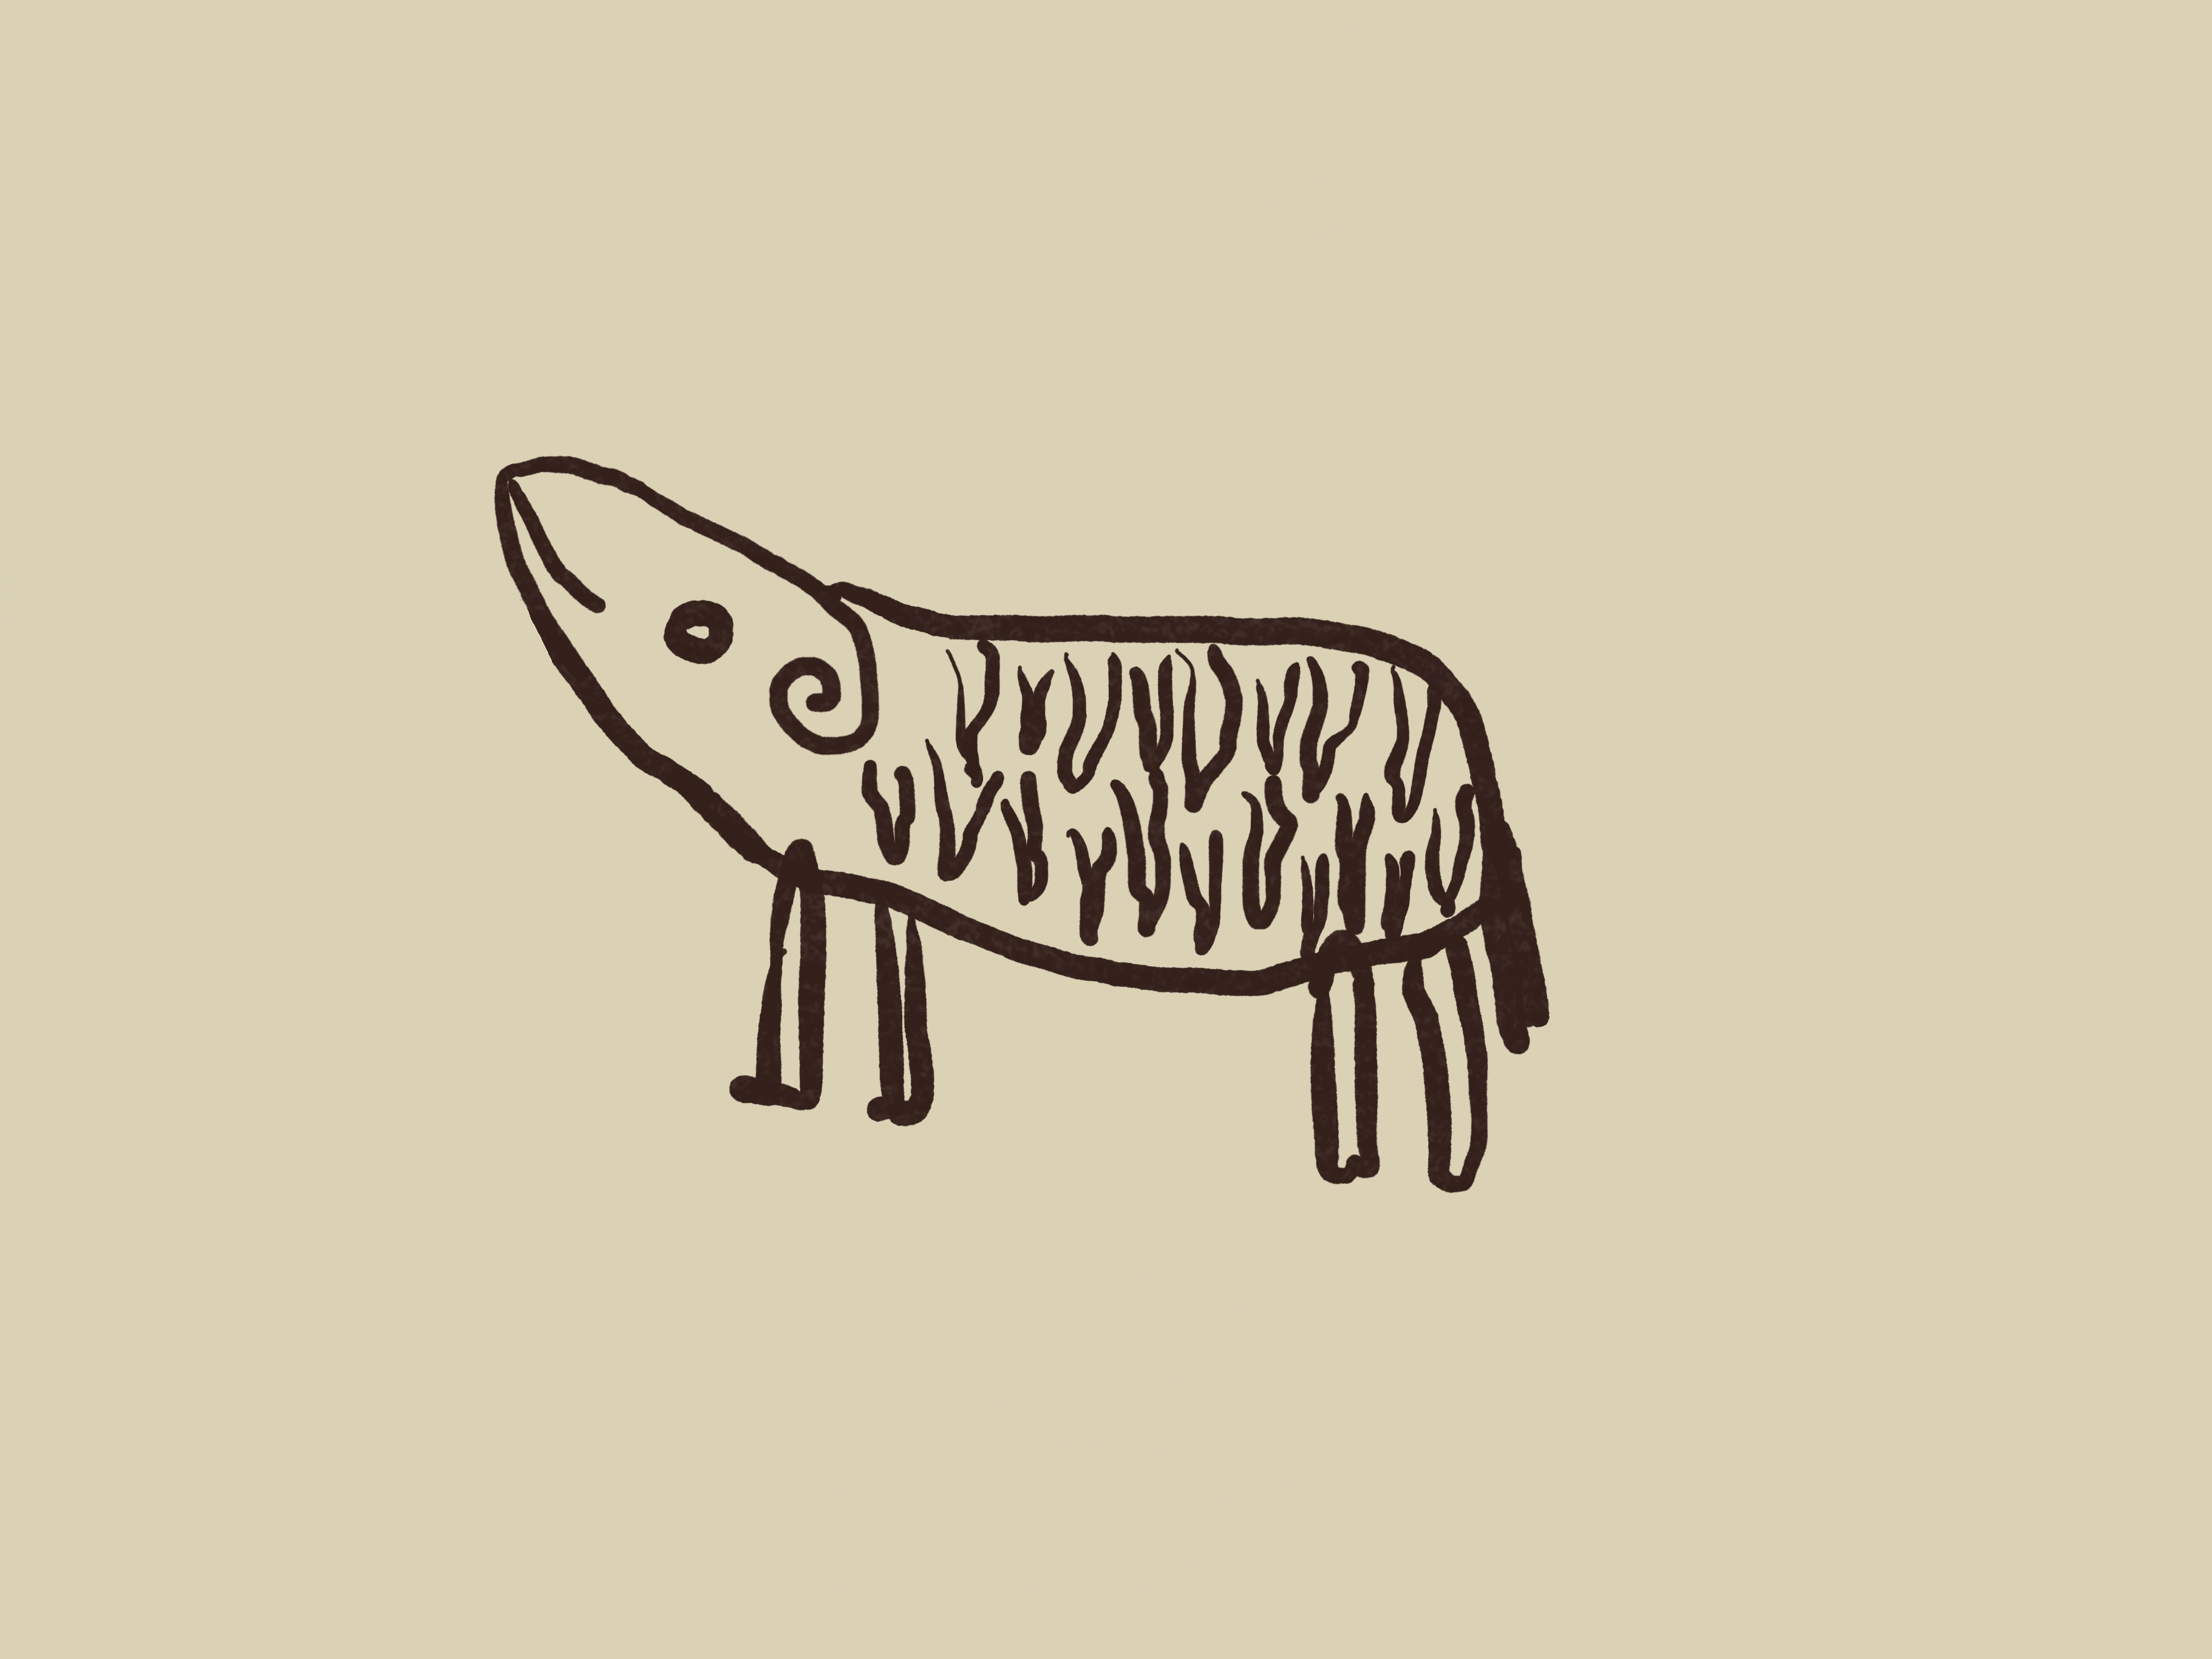
\includegraphics[width=1\textwidth,height=\textheight]{images/shesasheep.jpeg}
\end{center}

A Dissertation presented to the Graduate Faculty of the University of
Virginia in Candidacy for the Degree of Doctor of Philosophy

\paragraph{Department of French}\label{department-of-french}

\paragraph{University of Virginia}\label{university-of-virginia}

\paragraph{April 2025}\label{april-2025}

\bookmarksetup{startatroot}

\chapter{Abstract}\label{abstract}

This is where my abstract will go\ldots{}

\bookmarksetup{startatroot}

\chapter{Acknowledgements}\label{acknowledgements}

This is where my acknowledgements will go\ldots{}

\bookmarksetup{startatroot}

\chapter{Introduction}\label{introduction}

This is where my introdcution will go\ldots.

\bookmarksetup{startatroot}

\chapter{The Portraits}\label{the-portraits}

Each of these columns features an edited transcription and English
translation of the two portraits of Mary the Egyptian as they appear in
each of the T manuscripts. Copy T-L is not included on this page due to
lack of access to the original manuscript at the British Library. The
two fragmentary copies of Version T (T-F\textsuperscript{1} and
T-F\textsuperscript{2}) do not offer any lines of either portrait, and
so, they have also been excluded from this page.

To read these passages in translation, hover over each column with your
cursor.

\begin{figure*}

\section{T-A}\label{t-a}

\ldots.. De se biaute de se figure Si com ele est en escriture Vueil -i-
peu dire le samblant Anchois que je trespas avant Car a cel tans en icel
regne Ne vit nus hom plus bele feme Ne onc contesse ne roine Nen ot el
front plus bele crine Reondes avoit les oreilles Mais blanches erent a
merveilles Les iex clers \& sosrians les sorchix noir \& avenans bouche
petite par mesure \& pie le regardeiue Le face tenrre \& coloree Com le
rose qui sempre est nee Ja el nes ne el menton N'aperceussies mesfaichon
En som le col blanc com ermine li undoit le bloie crine Les mameles de
cele dame N'estoient menrres d'une pome Desous le goule en le poitrine
Ert blanche conme flor d'espine blans bras avoit \& blances mains Les
dois reons grailles \& plains Gent cors avoit \& bien molle Sous
l'aissele lonc le coste El n'iert trop grant no trop petite Ja se
faichon n'en iert escrite Ja le biaute de ceste dame Nen iert escrite
par nul home Tant iert cortoise de parler Riens n'i avoit que amender A
plaindre fait tel criaature Quant del Creator n'avoit cure El recevoit
plusors presens S'en acatoit bons vestemens Bons dras avoit . \& avenans
Por mix plaisir a ses amans Ele n'avoit soing de dras de lainne Au pior
jor de le semainne Bon bliaut avoit d'ostorin \& affubloit mantel
d'ermin Soullers bien pains de cordouam Cauchoit a tous les jors de l'an
Le citoien de le cite L'amoient tout por se biaute Li anchien home \& li
saige disoient tout Dex quel damage Com mar fu onc ceste dolante Tant
fait a plaindre se jovente Tant mar fu onques le siue vie Quant si est
plainne de folie Tout disoient par le cite Qu'ele estoit de haut parente
Car a tos respondoit raison \& tant iert bele de fachon ke li fix d'un
empereor Le peust prendre a grant honor \ldots.. Tant ala par jor \& par
nuit A faim \& a soif \& a dur lit Que tant parfont fu el boscaige Toute
devint illuec salvaige Mais ele ne s'oublioit mie De deprier sainte
Marie Sovent li menbroit de l'ymaige Que ele avoit mis en ostaige Si
souller furent tout use \& tout si drapel deschire Li cors de li remaint
tout nu N'avoit drapel ne fust rompu Li chars de li mua coulor Qui ains
iert blance conme flor Que por yver que por este Tout li noircirent li
coste Coulor mua se bloie crine Blanche devint com une hermine Le bouce
li fu tenevie \& environ toute noirchie \& avoit tant noir le menton
Conme s'il fust taint de carbon Atenerge furent li oel N'i avoit ore
point d'orguel Se vos veissies les oreilles Molt par vos presist grans
merveilles Car noire estoit \& decrevee Le blanche char toute muee Noire
\& muee ert le poitrine A escorce samblant d'espine N'avoit plus char en
ses traians Ne mais com il a en uns gans Les bras les mains \& les lons
dois Avoit plus noirs que nule pois Ongles avoit longes \& grans Ele les
retailloit a ses dens Li ventres li estoit caoit Petit de despensse i
metoit Li pie li erent decreve En plusors lius erent navre Car ele ne se
gardoit d'espine Quant ele aloit par le gastine Che li ert vis sien
esciant Que ele n'i failloit nient C'uns de ses pekies li caoit Quant
une espine le pongnoit Por chou estoit ele molt lie Quant ele souffroit
le hasquie N'est merveille se iert noirchie Car molt demenoit aspee vie
Plus de xl. ans ala nue N'iert merveille se iert moussue Povre despense
avoit o li Or ait Jhesus de li merchi .ii. pains avoit ne gaires grans
De chiaus vesqui par plusors ans El premier an devinrrent dur Com se
fust pierre de mur Cascun jor en usoit Marie Mais che iert petite partie
Quant ele ot tot son pain use Puis esrachoit l'erbe del pre Quant autre
beste le mengoit de rien ne se confortoit As mains buvoit l'iaue el
ruissel Quant ele n'avoit autre vaissel Ne font a plaindre li pechie
Dont li cors fu si castie D'erbe vesqui \& de rachines Xvii. ans. par
les gastines Puis fu .xxx. ans onc ne menga Se angeles ne li aporta Li
diables le an premier Le soloit sovent essaier Tout che li faisoit
remembrer Qu'ele soloit tos jors amer Les bons mengiers \& les biax
lieus Ou ele soloit faire les geus Or fu ichi boneuree Qu'ele de tout fu
obliee Onques puis en toute se vie Ne li souvint mais de folie Ne ainc
en trestot le boscaige Ne li vint puis beste salvaige Ne autre vive
creature Par le gaut va toute seure En plusors lius prist son ostel Se
vie ert tote esperitel \ldots..

\ldots.. Of her beauty, of her figure as it is in the written source I
want to say a little about her appearance before I go too far. For at
that time in that reign, no man saw a more beautiful woman. Never
countess nor queen had over her brow more beautiful hair. She had round
ears. What's more, they were marvelously white, her eyes bright and
smiling, her eyebrows black and becoming, her little mouth mild, and
pious her gaze, her face tender and blushing like the rose that is
always in bloom. Indeed neither on her nose nor on her chin would you be
aware of any defect. Her neck was white like ermine too. There flowed
her blonde hair. The breasts of this lady were no smaller than apples.
Above the cleavage of her chest, it was white like hawthorn flower. She
had white arms and white hands, her fingers shapely, slender, and
smooth. She had a fine body and well molded from her underarm along her
rib. She was neither too big nor too small. Her frame could never be
written. The beauty of this lady could never be written by any man. She
was so courteous of speech. There was nothing to improve. Such a
creature makes one lament when she does not care about the Creator. She
received many presents and bought herself good garments. She had good
and fitting clothes to better please her lovers. She did not care for
woollen cloth. On the worst day of the week, she had a fine purple silk
bliaut and adorned herself with an ermine mantle. Well-painted shoes of
Cordovan leather she put these on all the days of the year. The citizens
of the city loved her entirely for her beauty. The old men and the wise
would all say, ``God, what a shame! Oh alas evermore for this suffering!
There is much to bemoan of her youth. Alas evermore for her life as it
is so full of folly.'' Everyone in the city would say that she was of
high parentage for she answered all with reason and had such a beautiful
frame that the son of an emperor could have taken her with great honor.
\ldots.. So she went by day and by night hungry, thirsty, and on hard
beds. She was so deep in the wood that she became entirely wild there,
but she never forgot to pray to saint Mary. Often she remembered the
image on which she had made her pledge. Soon her shoes were worn out,
and soon her clothes were all torn up. Her body was left totally naked.
She did not have clothing that was not in tatters. Her own flesh changed
color, that which before was white like a flower. From winter as from
summer, her sides blackened entirely. The color of her blonde hair
changed. It turned white like an ermine. Her mouth was thinned, and all
around it blackened, and her chin was so black as though it were dyed
with charcoal. Thinned were her eyes. There was not a shred of pride
now. If you saw her ears, you would really take in a great marvel. for
they were black and cracked. Her white flesh changed entirely Black and
changed was her chest. It seemed like thorny bark. There was no more
flesh in her breasts, no more than there is in a glove. Her arms, her
hands, and her long fingers were blacker than any pitch. She had long
and large nails. She reshaped them with her teeth. Her stomach was
sunken. She put little provisions in there. Her feet were split. In many
places, they were wounded for she did not protect herself from thorns as
she went through the wilderness. It seemed to her, in her mind, she was
not wrong about this at all, that one of her sins fell away when a thorn
pricked her. For this, she was so pleased as she suffered hardship. It
was no marvel that she was blackened for she led such a severe life.
After more than forty years in the nude, it was no marvel she was wooly.
She had poor provisions with her. Pray, may Jesus have mercy on her. She
had two breads of no great size. On these, she lived for many years. In
the first year, they became hard as though they were building stones.
Each day, Mary ate some, but this was a small portion. As soon as she
had eaten up all her bread, then she plucked the grass nearby. Like
other beasts she ate it. She provided herself with nothing else. On her
hands, she drank the water from the stream as she had no other vessel.
She does not bemoan her sins as her body is so chastised. On grass she
lived and on roots for seventeen years in the wilderness. Then for
thirty years, she ate nothing unless an angel brought it to her. In the
first year, the devil often used to tempt her, making her remember all
that she used to always love. The good eats and the beautiful places
where she was used to playing games. Now, she was so blissful that she
had forgotten all. Never then in all her life did she think more of
folly. Never in all the wood did any wild beast come to her thereafter
nor any other living creature. Through the forest, she goes completely
safe. In many places, she took shelter. Her life was entirely spiritual.
\ldots..

\section{T-B}\label{t-b}

\ldots.. de sa biate de sa figure. si com ele est en l'escriture Vos
vuel dire de se senblant. ancois que je trespas avant Ans en cest mont
ne en cest regne. Ne vit nuz hom plus bele feme Onques ducoise ne roine.
ne n'ot el cief plus bele crine Reondes avoit les orelhes. Mais blanches
erent a mervelhes Les sorciz noirs \& avenanz. \& les olz clers \&
sorrianz La face tenre en celee.ee. Com la rose ki or est nee Les dens
ot blans \& bien menuz. plus bele boce ne vit nuz mut avoit piue
regardure. \& cler le vis \& le faiture Je cui el neis ne el menton.
n'avoit un point de mesfacon Soz la boce sor le poitrine. ert plus
blanche ke flors d'espine \& si avoit beles mameles. mut bien seans
petiz \& beles blans bras avoit \& blanches mains. \& les dois grailes
lons \& plains Gent cors avoit \& bien moleit. desoz l'aisselle \& le
costeit tant ert cortoise de parler n'i avoit rien ke amendeir N'ert pas
trop grant ne trop petite. Ja se facons n'en iert descrite Ja le beate
de ceste toise. N'iert descrite se n'i at proise a plendre fait tel
creature. cant de se Creator n'at cure ele recivoit grans presenz. s'en
achatoit chier garnimenz bon dras avoit \& avenanz. por miez plaissir a
ses amanz \& ne vestoit pas dras de laine. Le peior jor de la samaine
Vestoit bon bliat d'osterlin. \& affiebloit mantel d'ermin Solers biens
poins de corduan. chacoit par toz les jors de l'an Li citain de la
citeit. L'amoient tuit por sa bialteie \& li viel home \& li sage.
disoient tuit Deus kel damage tant mar fut iceste dolente. mut fait a
plendre sa jovente mar fut onques la sue vie. que tant est plane de
folie car a toz respondoit raison. tant ert de bele afaitison Que li fiz
d'un empereor. la poist prendre par honor \ldots.. tant errat par nuiz
\& par dis. a fain a soit \& a durs lis Que tant i fut en le boscage.
qu'ele devint tote salvage Senpres furent si drap useit. \& soi soler
tot depaneit tant par l'iver tant par l'esteit. tot li noicirent li
costeit Se tenre car muat color. qui ans eret blance cum florr Color
muat sa bele crine. blance devint conme l'ermine desoz la face eret
brulee. del soloilh \& de la jalee La boche li ert atenevie. \& environ
la cars norcie \& tant avoit noir le menton. com se fuist li chies d'un
tison atenevit erent li oilh. or n'i avoit il point d'orgoilh se vos en
veissiez l'orelhe mut vos venist a grant mervelhe car maigre ert mut \&
degregue. \& de blanc poilh tote mossue Noire \& polhue ert la poitrine.
sembloit scorce de noire spine Li ventres li ert toz caoiz. nient ne
manjoit \& si ert droiz Les ongles avoit ele granz. ele les retalloit az
danz Les piez maigres \& decrevez. \& par plusors lius mut navrez car
ele nes gardoit d'espine. cant el aloit par le gastine Ans li ert vis
son escient. \& ele ni faloit nient cant une spine li poindoit. uns des
pechiez jus li chaoit Ne fat a plaindre li pechiez. dont li cors est si
castoiez N'ert mervelhe s'ele ert mossue. karante ans alat tote nue Dous
pains avoit ne gaire granz. de ces viscat par plusors anz Le premier an
devinrent dur. com ce fust piere de mur cascun jor en usoit Marie. mais
ce astoit mut povre vie cant ele ot toz ses pains useiz. puis esragat
herbes des prez com altre beste le manjoit. de rien ne se desconfortoit
Ades bevoit ens el ruisel. ele n'avoit altre vaissel d'erbes vivoit \&
de racines. dis \& uit ans par la gastines Puis fut vint ans que ne
manja. sel angeles Deu ne li porta Diables li vint devant premier. que
mut le soloit anoier que li faissoit ramembrer. kanque soloit jadis
ameir Les biaz deliz \& les biaz giuz. u soloit faire ses deduiz Mut fut
bieneuree. ki de tot ce fut obliee unques puis en la sue vie. Ne li
menbra jor de folie Marie vat par le boscage. Onques n'i vit beste
salvage Ne nule vive creature. par le forest vat bien segure en plusors
lius fut ses ostaz. sa vie astoit spirituaz \ldots..

\ldots.. Of her beauty, of her figure as it is in the written source I
want to tell you about her appearance. before I go too far. In this
world and in this reign, no man saw a more beautiful woman. Never
duchess nor queen had on her head more beautiful hair. She had round
ears. What's more, they were marvelously white, her eyebrows black and
becoming, and her eyes bright and smiling, her face tender and covered
like the rose that has only just bloomed. Her teeth were white and quite
small. A more beautiful mouth no one ever saw. She had such a pious
gaze, and her look and her features bright. I believe on her nose and on
her chin there was no defect at all. Above the bump on her chest, it was
whiter than hawthorn flower, and of course she had beautiful breasts, so
well set, small, and beautiful. She had white arms and white hands, and
her fingers slender, long, and smooth. She had a fine body and was well
molded beneath her underarm and her rib. She was so courteous of speech.
There was nothing to improve. She was neither too big nor too small. Her
frame could never be described. The beauty of these proportions could
neither be described nor appraised Such a creature makes one lament when
she does not care about her Creator. She received great presents and
bought herself expensive garments. She had good and fitting clothes to
better please her lovers, and she did not wear woollen cloth. The worst
day of the week, she wore a fine purple silk bliaut and adorned herself
with an ermine mantle. Well-painted shoes of Cordovan leather she put
these on all the days of the year. The citizens of the city loved her
entirely for her beauty, and the old men and the wise would all say,
``God, what a shame! Alas for this suffering! There is much to bemoan of
her youth. Alas evermore for her life is so full of folly.'' As she
answered all with reason and had such a beautiful frame, the son of an
emperor could have taken her with honor. \ldots.. So she roamed by night
and by day hungry, thirsty, and on hard beds. Like that, there she was
in the wood, and so, she became entirely wild. Soon, her clothes were
worn out, and soon her soles were torn up. As much from winter as from
summer, her sides blackened entirely. Her tender flesh changed color,
which before was white like a flower. The color of her beautiful hair
changed. It turned white like the ermine. Under that, her face was
burned from the sun and from the frost. Her mouth was thinned, and her
flesh around it blackened, and her chin was so black as if it were the
head of a firebrand. Thinned were her eyes. There was not a shred of
pride now. If you saw her ears, you would come upon a great marvel for
they were so skinny and degraded and all wooly with white hairs. Black
and hairy was her chest. It seemed like black thorny bark. Her stomach
was all sunken. She ate nothing and so that was right. She had large
nails. She reshaped them with her teeth. Her feet were skinny and split,
and in many places were so wounded for she did not protect them from
thorns as she went through the wilderness. So it seemed to her, in her
mind, and she was not wrong about this at all, as a thorn pricked her,
one of her sins fell down from her. She does not bemoan her sins as her
body is so chastised. It was no marvel that she was wooly; for forty
years, she went totally nude. She had two breads of no great size. On
these, she lived for many years. The first year they became hard as
though they were building stone. Every day, Mary ate some, but this was
a very poor life. As soon as she had eaten up all her bread, then she
went wild for the grasses nearby Like other beasts, she ate them. She
provided herself with nothing else. She drank from the stream all the
time. She had no other vessel. On grasses she lived and on roots for
eighteen years in the wilderness. Then for twenty years, she only ate
what the angel of God brought to her. The devil came before her first.
He used to annoy her so much making her remember whatever she once used
to love, the beautiful delights and the beautiful games in which she
used to take pleasure. She was so blissful that she had fogotten all of
this. Never again in her life did she bring to mind a day of folly. Mary
goes through the wood. Never did she see a wild beast nor any living
creature. Through the forest, she goes so secure. In many places, she
was sheltered. Her life was spiritual. \ldots..

\section{T-C}\label{t-c}

\ldots.. De sa beaute de sa figure Si cum il est en escripture . Voil un
poi dire le semblant Ainz co ke jo pas avant . A iceu tens n'ert si bele
femme kar ele estoit sur tutes gemme . Onke cuntesse ne reine N'ot el
chief si bele crine . Rondes avoit les oreilles Tres blanches erent a
merveilles . Les surcius noirs e avenanz e les oils clers e suz rianz .
La buche petite par mesure e simple avoit la regardure . La face tendre
e coluree Cum rose qui sempres est nee . Ne ja au nes n'au mentun
N'aparceussez meffacon . Par sum le col blanc com ermine Lui undoit la
bloie crine . Chascun des traianz la dame N'iert pas maire d'une pome .
Suz la gule en la peitrine ert blanche come fleur d'espine . Lung braz
avoit e blanche mains Les dois ronz.greilles e pleins . Gent cors avoit
e bien moullez Desuz l'essele les long costez . Ne feut trop grant ne
trop petite Sa facon n'iert ja descrite . Ne la beaute de ceste dame
N'iert ja descrite pur nul aume . Tant ert cortoise de parler Riens n'i
avoit k'amender . A pleindre fist teu creature Quant de sun Creatur n'ot
cure . ele recevrit mut presenz S'en achatot beau vestemenz . Bons dras
avoit e avenanz Pur menz pleire a ses amanz . ele n'avoit soign de dras
de leine Par nul des jurs de la sumeine . Ainz vesteit bliauz de osterin
e affublout mantel d'ermin . Sollers bien peinz de cordewan Chaucot
trestuz les jurs del an . Trestuz cous de la cite L'amoient pur la
beaute . Li ancien hom e li sage Disoient. hai. queu damage . Tant mar
fu nee la dolente Tant fet a pleindre sa juvente . Mar feut onke la sue
vie Quant si est pleine de folie . Tuz diseient par la citez k'ele
estoit de grant parentez . kar a tuz respont par reison e tant ert bele
de fascon . ke li fiz d'un empereur La peust prendre a gran honur .
\ldots.. Tant alad ke jurs ke nuiz Od feims od seifs \& od dur liz . ke
tant parfond feut en boscage Tote devint illoec salvage . mes ele ne
s'obliat mie De deprier saincte Marie . sovent li membre de l'ymage
k'ele avoit mis en hostage . si drapel furent tost usez e si souler tut
deramez . kant li drapel erent rumpu Le cors de lui remist tut nu . La
char de lui mua colur k'einz ert blanche come flur . ke de l'yver ke de
l'este Tut li nercirent li coste . Colur muat la bloie crine Blanche
devint com ermine . La face lui estoit bruillee Del grant soleil e de
gelee . La buche li ert entenvie e d'environ tote en nercie . e tant
avoit neir le menton come co feust chief d'un tison . Teint e nerci
erent li oil Rien n'i ot ore d'orgoil . se vos regardisez s'oreille mut
vos serroit grant merveille . car megres estoit e descrue e de blanc
peil tote mossue Noire e mossue ert la peitrine L'escorce semblout
d'espine . N'avoit plus char en sa triant Ne mes ke n'ad en un gant .
Les braz les mains e les lung dois Avoit plus noirs ke nule poiz . Les
ungles avoit ele mut grenz Si les retaillot de ses denz . Li ventre tut
lui ert caeiz Guere ne mangot. co ert droiz . Les piez lui erent
escrevez en plusur lius furent nafrez . k'ele ne se gardoit d'espine
kant ele alot par la guastine . Co lui ert vis son escient Pur voir de
co ne failli nient . k'un de ses pechiez chaeit kant une espine la
puigneit . Pur co feut ele mut lee kant ele suffri teu haschee . N'ert
merveille se feust nercie ke mut demenot aspre vie . plus de quarante
anz ala nue Ne fu merveille s'ert mossue . Povre despense avoit od lui
Ore ait de lui Jhesu merci . Dous pains avoit ne guere granz De ces se
garit plusurs anz . Tut al premor devindrent dur Cum s'il feusent fet de
mur . Chescun jor en usout Marie mes co ert petite partie . kant ele out
son pain use Doncs arracot l'erbe du pre . Com autre beste la mangot De
rien ne se desconfortout . Adenz leveit un rosel Dont beut n'ot autre
vessel . Ne fet a pleindre le pechie Dont le cors fu si chastie . D'erbe
vesquit e de racine Dis e ut. anz en la gastine . pus fu trente anz onc
ne manga si l'angle Deu ne lui porta . Diables la veneient esprimer
Sovent la soleient assaer . Tut co lui firent remembrer k'ele soleit ja
dis amer . Les bons mangers e les beau lius Ou ele soleit fere ses gius
. Lors feut ele si bonureie ke de rien n'ert attameie . unk en tote soue
vie Ne lui sovint puis de folie . Ne puis en trestut le boscage Ne vit
guere beste sauvage . N'autre vive creature Par la forest vait tute sure
. en plusur lius prent son hostal Sa vie est tute espirital . \ldots..

\ldots.. Of her beauty, of her figure as it is in the written source I
want to say a little about her appearance before I go on. At that time,
there was no woman so beautiful for she was a gem above them all. Never
countess nor queen had on her head such beautiful hair. She had round
ears. They were very marvelously white, her eyebrows black and becoming,
and her eyes bright and overjoyed, her little mouth mild, and she had a
simple gaze, her face tender and blushing like a rose that is always in
bloom. Indeed neither on her nose nor on her chin would you be aware of
any defect. Along her neck was white like ermine. There flowed her
blonde hair. Each of the breasts of the lady was no more than an apple.
Above the cleavage of her chest, it was white like hawthorn flower. She
had long arms and white hands, her fingers shapely, slender, and smooth.
She had a fine body and was well molded from her underarm along her rib.
She was neither too big nor too small. Her frame could never be
described. Nor could the beauty of this lady ever be described by any
man. She was so courteous of speech. There was nothing to improve. Such
a creature makes one lament when she does not care about her Creator.
She received many presents and bought herself beautiful garments. She
had good and fitting clothes to better please her lovers. She did not
care for woollen cloth. On any of the days of the week, she wore her own
bliaut of fine purple silk and adorned herself with an ermine mantle.
Well-painted shoes of Cordovan leather, she put these on all the days of
the year. Every man of the city loved her for her beauty. The old men
and the wise would say, ``Ah! What a shame! Alas was born suffering!
There is much to bemoan of her youth. Alas evermore, her life is so full
of folly.'' Everyone in the city would say that she was of great
parentage for she answered all with reason and had such a beautiful
frame that the son of an emperor could have taken her with great honor.
\ldots.. So she went in the day as in the night hungry, thirsty, and on
hard beds. She was so deep in the wood that she became entirely wild
there, but she never forgot to pray to saint Mary. Often she remembered
the image on which she had made her pledge. Soon her clothes were worn
out and soon her soles were stripped. As her clothes were in tatters,
her body was left totally naked. Her own flesh changed color, that which
before was white like a flower. From the winter and from the summer her
sides blackened entirely. The color of her blonde hair changed. It
turned white like ermine. Her face was burned by the blazing sun and by
the frost. Her mouth was thinned and all around it blackened, and her
chin was so black it was like the head of a firebrand. Tinted and
blackened were her eyes. There was not any pride there now. If you saw
her ears, they would really be to you a great marvel for they were
skinny and cracked and all wooly with white hairs. Black and wooly was
her chest. It seemed like thorny bark. She had no more flesh in her
breast, no more than there is in a glove. Her arms, her hands, and her
long fingers were blacker than any pitch. She had such large nails. So
she reshaped them with her teeth. Her stomach was all sunken. She hardly
ate, so that was right. Her feet were split. In many places, they were
wounded for she did not protect herself from thorns as she went through
the wilderness. It seemed to her, in her mind, for truly, about this,
she was not wrong at all, that one of her sins fell away when a thorn
pricked her. For this, she was so pleased. As she suffered such
hardship, it was no wonder that she was blackened for she led such a
severe life. After more than forty years in the nude, it was no wonder
she was wooly. She had poor provisions with her. Pray, may Jesus have
mercy on her. She had two breads of no great size. On these she
sustained herself for many years. They all became hard in the first year
as though they were made from a wall. Each day, Mary ate some, but this
was a small portion. As soon as she had eaten up her bread, then she
gathered the grass nearby. Like other beasts she ate it. She provided
herself with nothing else. Prone, she drew from a stream. Like so, she
drank. She had no other vessel. She does not bemoan her sins as her body
was so chastised. On grass she lived and on roots for eighteen years in
the wilderness. Then for thirty years, she never ate but what the angel
of God brought to her. Devils came to approach her. Often they used to
tempt her, making her remember all that she once used to love. The good
eats and the beautiful places where she was used to playing her games.
Now, she was so blissful that nothing hurt her. Never, in all her life,
did she think, then, of folly. Nor, then, in all the wood, did she see
wild beasts at all. nor any other living creature. Through the forest,
she goes totally sure. In many places, she takes shelter. Her life is
entirely spiritual. \ldots..

\section{T-D}\label{t-d}

\ldots.. De sa bealte \& de sa figure Si cum est en l'escripture voil un
poi dire le semblant einz que jeo trespas avant en cel tens ne en cel
regne Ne vit unc home plus bele femme Ne cuntesse ne raine. N'out onkes
tele meschine roundes avoit les oreilles Mais blanches erent a
merveilles les sorciz neirs \& avenanz les oilz neirs \& sorianz la
bouche brieve \& par mesure \& pie la regardeure la face tendre \&
coloree cumme rose qui senpres est nee ja el nes ne el mentun N'i veist
l'un mesfacun par sun le col blanc cum ermine li undout la bloie crine
chascun des traianz a la dune N'ert mie greignor d'une pume Soz la gorge
en la poitrine ere blanche cumme flor d'espine blans bras aveit \& beles
mains \& les deis luncs gresles \& pleins N'ert trop grande ne trop
petite ja sa facun n'iert deserite ja la bealte de ceste dune N'iert
escrite por nul home tant ert corteise de parler rien n'i aveit que
amender a plaindre fait tel creature Quant del Creator n'aveit cure ele
recevoit or \& argent Si achatout bons garnemenz bons dras aveit \&
avenanz por miex plesir a ses amanz ele n'out cure de dras de leine al
peor jor de la semeine Vesteit bons bliaus d'osturin \& afubla mantel
hermin Soulers bien pains de cordouen chaucout a toz les jors de l'an li
citeen de la cite l'amouent tuit por sa bealte li anciem home \& li sage
disoient tuit Deus quel damage Mar fu unques la dolente tant fait a
plaindre sa jovente Mar fu unques la soue vie Quant si est pleine de
folie tuit disoient par la cite Que ele ert de mult halt parente car a
toz rosponeit raisun \& tant ert bele de facun ke le fiz d'un enpereor
la peust prendre par honor \ldots.. tant erra par jor. \& par nuit o
faim. \& o sei. \& o dur lit \& tant fu en cel boscage tote devint iloc
salvage mais ele ne s'oublia mie de deprier sainte Marie sovent lui
membre de l'ymage Que ele aveit mis en ostage Ses soulers furent tuit
uses \& si drapel tuit descires Quant si drapel furent rumpu le cors de
lui remist tot nu la char de lui mua color Qui ainz ert blanche cumme
flor Que o l'ivern. ke o l'este tuit li nercirent li coste color mua sa
bloie crigne blanche devint cumme ermigne la face out desus bruslee del
soleil. \& de la gelee la bouche li fu atenvie \& envirun la char nercie
tant par esteit noir sun mentun. cum ceo fust le chief d'un tisun \&
nerci erent si oil N'i aveit ore point d'orguil Se vous veisses sa
oreille mult vous semblast grant merveille car mesgre esteit. \&
detrevee \& de blanc peil avirunee N'aveit plus char en sun traiant Ne
mais cum il a en un gant les bras. les mains. \& les deiz aveit plus
neirs que nule peiz les ongles aveit ele grenz ele les taillout o les
denz le ventre lui ert tot dechaet car povre despense i meteit les piez
li erent decrevez en plusors lieus erent nafrez car ele ne se gardout de
espine Quant ele alout par la gastine mais ceo li ert vis son encient \&
ele n'i failli de nient ke un peche de lui chaeit Quant une espine la
poingneit por ceo esteit ele lee Quant ele soffri une haschee N'ert pas
merveille s'ele ert nercie car ele demenout aspre vie plus de quarante
ans ala nue N'ert merveille s'ele ert mossue povre despense aveit o lui
ore ait Jesus de lui merci deus pains aveit ne gueres granz de cels
vesqui plusors anz el premier en devindrent dur cumme ceo fussent pieres
de mur chascun jor en usout Marie mais ceo ert petite partie \& quant
ele out son pain use Si esracout l'erbe del pre cumme altre beste la
manjout \& de rien ne se desconfortout a denz beveit del ruissel ele
n'aveit altre vaissel Ne fait a plaindre le pechie dunt le cors fu si
chastie d'erbes viveit. \& de racines dis. \& set anz. en la gastine
puis fu trente anz unc ne manja Se li angres Deu ne lui porta deable lui
vint de premier Sovent la soloit essaier tot ceo lui faisoit remembrer
Que ele soloit jadis amer les bons mangiers. \& les lieus ou ele sout
faire ses gieus ore fu issi beneuree Que de tot ceo fu obliee \& en tote
la soue vie Ne lui sovint puis de la folie \& unc puis en tot le boscage
Ne vit beste salvage Ne altre vive creature par la forest vait tote
seure en plusors lieus prent son ostal Sa vie esteit esperital \ldots..

\ldots.. Of her beauty and of her figure as it is in the written source
I want to say a little about her appearance before I go too far. At that
time and in that reign, no man ever saw a more beautiful woman. No
countess or queen ever had such a daughter. She had round ears, what's
more, they were marvelously white, her eyebrows black and becoming, her
eyes black and smiling, her mouth small and mild, and pious her gaze,
her face tender and blushing like a rose that is always in bloom. Indeed
neither on her nose nor on her chin was seen a defect. Along her neck
was white like ermine. There flowed her blonde hair. Each of the breasts
of the lady was not a bit bigger than an apple. Above the cleavage of
her chest, it was white like hawthorn flower. She had white arms and
beautiful hands, and long, slender, and smooth fingers. She was neither
too big nor too small. Her frame could never be described. The beauty of
this lady could never be written by any man. She was so courteous in
speech. There was nothing to improve. Such a creature makes one lament
when she does not care about the Creator. She received gold and silver
and bought good garments. She had good and fitting clothes to better
please her lovers. She did not care for woollen cloth. On the worst day
of the week, she wore a fine purple silk bliaut and adorned herself with
an ermine mantle. Well-painted shoes of Cordovan leather, she put these
on all the days of the year. The citizens of the city loved her entirely
for her beauty. The old men and the wise all would say, ``God, what a
shame! Alas evermore, the suffering! There is much to bemoan of her
youth. Alas evermore, her life is so full of folly.'' Everyone in the
city would say that she was of such high parentage for she answered all
with reason and had such a beautiful frame that the son of an emperor
could have taken her with honor. \ldots.. So she roamed by day and by
night, hungry and thirsty and on hard beds, and so she was in this wood.
She became entirely wild there, but she never forgot to pray to saint
Mary. Often, she remembers the image on which she had made her pledge.
Her soles were all worn out, and soon her clothes were torn up. As her
clothes were in tatters, her body was left totally naked. Her own flesh
changed color, that which before was white like a flower. From the
winter and from the summer her sides blackened entirely. The color of
her blonde hair changed. It turned white like ermine. Her face was
burned up from the sun and from the frost. Her mouth was thinned, and
her flesh around it blackened. Her chin was so black all over. It was
like the head of a firebrand, and black were her eyes. There was not a
shred of pride now. If you saw her ears, they would really seem to you a
great marvel for they were skinny and cracked and covered in white hair.
She had no more flesh in her breast, no more than there is in a glove.
Her arms, her hands, and her fingers were blacker than any pitch. She
had large nails. She shaped them with her teeth. Her stomach was all
sunken for she put poor provisions in there. Her feet were split and, in
many places, were wounded for she did not protect herself from thorns as
she went through the wilderness. But it seemed to her, in her mind, and
she was not wrong about this at all, that a sin fell away from her when
a thorn pricked her. For this, she was pleased. As she suffered
hardship, it was no wonder she was blackened for she led a severe life.
After more than forty years in the nude, it was no wonder she was wooly.
She had poor provisions with her. Pray, may Jesus have mercy on her. She
had two breads of no great size. On these, she lived for many years. In
the first year, they became hard as though they were building stones.
Each day, Mary ate some, but this was a small portion. And as soon as
she had eaten up her bread, then she plucked the grass nearby. Like
other beasts, she ate it. And she provided herself with nothing else.
Prone, she drank from the stream. She had no other vessel. She does not
bemoan her sins as her body was so chastised. On grasses she lived and
on roots for seventeen years in the wilderness. Then, for thirty years,
she never ate but what the angel of God brought to her. The devil came
to her first. Often he used to tempt her, making her remember all that
she once used to love. The good eats and the places where she was used
to playing her games. Now, she was so blissful as she had forgotten all
of this. And in all her life, she never thought of folly. And never then
in all the wood did she see any wild beast nor any other living creature
Through the forest, she goes totally sure. In many places, she takes
shelter. Her life was spiritual. \ldots..

\section{T-E}\label{t-e}

\ldots.. de sa bieute de sa figure Si com il est en escripture Voil -i-
poi dire le samblant ancois que jo trespas avant En icel tans ne en cel
regne N'en ot onques plus bele feme onques comtesse ne roine Nen ot el
chief plus bele crigne rondes avoit les oreilles \& blances erent a
merveilles les sorcils nois \& avenans \& les ioex vairs \& molt rians
La bouche bele \& par mesure \& pieue la regardeure la face tenre \&
coloree comme rose novele nee Ne ja el nes ne el menton Ne parceuscies
mesfacon Le col avoit blanc com ermine Loiet estoit sa blonde crine
N'iert mie greindres d'une pome L'un des traians de cele domme desus la
boce en la poitrine Ert si blance com flor d'espine blans bras avoit \&
blances mains les dois reons greilles \& plains Gent cors avoit \& bien
molle Sus l'asoele lanc le coste Ne trop grande ne trop petite Ja sa
facon n'en ert descrite la grans biautes de ceste dame N'iert toute
escrite par nul homme Tant ert cortoise de parler Rien n'i avoit que
amender a plaindre fait tel creature Quant de son Creator n'a cure Ele
recevoit grans presens S'en achatoit biaus garnemens biaus dras avoit \&
avenans por bien plaisir a ses amans N'avoit pas soing de dras de laine
Al pior jor de la semaine vestoit bon bliaut ostorin Si afubloit mantel
ermin Sollers bien pains de cordoan chaucoit a tus les jors del an li
citeain de la cite l'amoient tot por sa biaute li ancien home \& li sage
disoient tot que cert damage tant par mar fu ceste dolente molt fait a
plaindre sa jovente mar fu onques la soie vie Quant si est plaine de
folie tot disoient par la cite Qu'ele ert de haut parente Car a tos
respondoit raison \& molt ert de bele facon li fiex a -i- empereor Le
peust prendre par honor \ldots.. tant ala par jor \& par nuis par bos
par plains \& par larris \& tant par font vint el boscage Que tot devint
iluec salvage mais ele ne s'oblioit mie de proier a sainte Marie Sovent
li menbroit del image Que ele avoit mis en ostage Si drapel furent tost
use \& si sollers tost desrame Quant si drapel furent ronpu li cors de
li remest tot nu la sieue char mua color devant ert blance comme flor
Quant .i. iver i ot este tot li noircirent li coste molt li mua la
blonde crine blance devint com .i. ermine del soleil \& de la gelee li
fu la face molt bruslee Sa bouche fu atenevie \& environ sa char noircie
itant avoit noir le menton comme ce fust chies d'un tison tot li erent
noir oi li oil N'avoit ore .i. point d'orgoil Se vos en veiscies
l'oreille molt vos venist a grant merveille Qui maigre estoit \& decreue
\& de blanc poil tote molsue Noire \& molsue ert sa poitrine bien
resambloit escorce d'espine N'avoit de char en ses traians Nient plus
qu'il est en .i. gans les bras les mains \& les lons dois Avoit plus
noirs que n'en est pois molt par avoit les ongles grans as dens les ront
qu'ele ot trencans li ventres li ert agaris car n'avoit nul de ses delis
li pie li erent decreve \& environ tot denavre Ele ne se gardoit
d'espine Quant ele aloit par la gastine Ce li ert vis son escient del
bien faisoit petit u nient Quant une espine le poignoit En un de ses
pies li chaoit de co estoit ele molt lie Quant ele avoit la grant hascie
N'estoit merveille s'iert noircie car molt demenoit aspre vie plus de
.xl. ans a la nue N'iert par merveille s'iert mossue povre despens avoit
od li Damedex ait de li merci .ii. pains avoit ne gaires grans de ces
vesqui par pluisors ans le premer an devindrent dur com ce fuissent
pieres de mur chascun jor en usoit Marie mais co ert petite partie Quant
ele ot tot son pain use donques aquelt l'erbe del pre com autre beste le
mangoit de rien ne se recomfortoit as dens bevoit dou ruissel Car n'i
avoit autre vaiscel Ne fait a plaindre li pechiet dont li cors est si
castiet d'erbe vesqui \& de racine dis \& set anz en la gastine puis fu
.xxx. anz que ne manga Se l'angles Deu ne l'aporta dyable vint a li de
premier Sovent le soloit assaier tot ce li faisoit ramenbrer Qu'ele ja
dis soloit amer les biaus delis \& les bels lieus ou ele seut faire ses
gieus ore fu ele boneuree Quant de tot ce fu obliee Ainc gaires puis en
tote sa vie Ne li sovint puis de folie Ne ainc en trestot le boscage Ne
vit gaires beste salvage Ne autre vive creature par la forest vait tote
nue En pluisors lieus prist son ostal Sa vie estoit esperital \ldots..

\ldots.. Of her beauty, of her figure as it is in the written source I
want to say a little about her appearance before I go too far. At that
time and in that reign, there was never a more beautiful woman. Never
countess nor queen had on her head more beautiful hair. She had round
ears, and they were marvelously white, her eyebrows black and becoming,
and her eyes sparkling and joyful, her mouth beautiful and mild, and
pious her gaze, her face tender and blushing like a freshly-bloomed
rose. Indeed neither on her nose nor on her chin might you perceive any
defect. Her neck was white like ermine. Long was her blonde hair. Not a
bit bigger than an apple were either of the breasts of this lady. Above
the bump of her chest, it was as white as hawthorn flower. She had white
arms and white hands, her fingers shapely, slender, and smooth. She had
a fine body and was well molded from her underarm along her rib. Neither
too big nor too small, her frame could never be described. The great
beauty of this lady could not be written fully by any man She was so
courteous in speech. There was nothing to improve. Such a creature makes
one lament when she does not care about her Creator. She received great
presents, and bought herself beautiful garments. She had beautiful and
fitting clothes to please her lovers well. She did not care for woollen
cloth. On the worst day of the week, she wore a fine purple silk bliaut
and adorned herself with an ermine mantle. Well-painted shoes of
Cordovan leather, she put these on all the days of the year. The
citizens of the city loved her entirely for her beauty. The old men and
the wise all would say that it was a shame. ``Alas for this suffering!
There is much to bemoan of her youth. Alas evermore, her life is so full
of folly.'' Everyone in the city would say that she was of high
parentage for she answered all with reason and had such a beautiful
frame. The son of an emperor could have taken her with honor. \ldots..
So she went by day and by night through woods, through plains, and
through hills, and so deeply she went into the wood that she became
entirely wild there, but she never forgot to pray to saint Mary. Often
she remembered the image on which she had made her pledge. Soon her
clothes were worn out, and soon her soles were stripped. As her clothes
were in tatters, her body was left totally naked. Her own flesh changed
color. Before, it was white like a flower. In winter as in summer, her
sides blackened entirely. Her blonde hair changed greatly. It turned
white like an ermine from the sun and from the frost. Her face was so
burned. Her mouth was thinned, and her flesh around it blackened. Her
chin was so black. It was like the head of a firebrand. All black were
her eyes now. She had, now, not a shred of pride. If you saw her ears,
you would come upon a great marvel that was skinny and cracked and all
wooly with white hairs. Black and wooly was her chest. It so ressembled
thorny bark. She did not have flesh in her breasts, nothing more than
there is in a glove. Her arms, her hands, and her long fingers were
blacker than pitch. She had such large nails on her slicing teeth she
made them round. Her stomach was sunken for she had none of her
delights. Her feet were split and wounded all over. She did not protect
herself from thorns as she went through the wilderness. It seemed to
her, in her mind, that it would do little or no good for as a thorn
pricked her in one of her feet, it would fall away. For this, she was so
pleased. As she bore great hardship, it was no wonder she was blackened
for she led a very severe life. After more than forty years in the nude,
it was no wonder she was wooly. She had poor provisions with her. May
God have mercy on her. She had two breads of no great size. On these she
lived for many years. The first year, they became hard as though they
were building stones. Each day, Mary ate some, but this was a small
portion. As soon as she had eaten up all her bread, then she gathered
the grass nearby. Like other beasts, she ate it. She provided herself
with nothing else. Prone, she drank from the stream for there was no
other vessel. She does not bemoan her sins as her body is so chastised.
On grass she lived and on roots for seventeen years in the wilderness.
Then, for thirty years, she ate only what the angel of God brought to
her. The devil came to her first. Often he used to tempt her, making her
remember all that she once used to love. The beautiful delights and the
beautiful places where she was used to playing her games. Now, she was
blissful as she had forgotten all of this before long. Then for all her
life, she never thought of folly. Never in all the wood did she see any
wild beasts at all nor any other living creature. Through the forest,
she goes utterly naked. In many places, she took shelter. Her life was
spiritual. \ldots..

\bookmarksetup{startatroot}

\chapter{The Portraits (with
Visualizations)}\label{the-portraits-with-visualizations}

ADD EXPLANATION OF VISUALIZATIONS

To read these passages in translation, hover over each column with your
cursor.

\begin{figure*}

\begin{figure}

\begin{minipage}{0.20\linewidth}

\section{T-A}\label{t-a-1}

\ldots.. De se biaute de se figure Si com ele est en escriture Vueil -i-
peu dire le samblant Anchois que je trespas avant Car a cel tans en icel
regne Ne vit nus hom plus bele feme Ne onc contesse ne roine Nen ot el
front plus bele crine Reondes avoit les oreilles Mais {blanches} erent a
merveilles {Les iex {clers} \& sosrians} {les sorchix {noir} \& avenans}
bouche petite par mesure \& pie le regardeiue Le face tenrre \&
{coloree} {Com le rose qui sempre est nee}

Ja el nes ne el menton N'aperceussies mesfaichon En som le col {blanc
com ermine} li undoit le {bloie} crine Les mameles de cele dame
N'estoient menrres d'une pome Desous le goule en le poitrine Ert
{blanche conme flor d'espine} {blans bras} avoit \& {blances mains} Les
dois reons grailles \& plains Gent cors avoit \& bien molle Sous
l'aissele lonc le coste El n'iert trop grant no trop petite Ja se
faichon n'en iert escrite Ja le biaute de ceste dame Nen iert escrite
par nul home Tant iert cortoise de parler Riens n'i avoit que amender A
plaindre fait tel criaature Quant del Creator n'avoit cure El recevoit
plusors presens S'en acatoit bons vestemens Bons dras avoit . \& avenans
Por mix plaisir a ses amans Ele n'avoit soing de dras de lainne Au pior
jor de le semainne Bon bliaut avoit {d'ostorin} \& affubloit mantel
d'ermin Soullers {bien pains} de cordouam Cauchoit a tous les jors de
l'an Le citoien de le cite L'amoient tout por se biaute Li anchien home
\& li saige disoient tout Dex quel damage Com mar fu onc ceste dolante
Tant fait a plaindre se jovente Tant mar fu onques le siue vie Quant si
est plainne de folie Tout disoient par le cite Qu'ele estoit de haut
parente Car a tos respondoit raison \& tant iert bele de fachon ke li
fix d'un empereor Le peust prendre a grant honor \ldots.. Tant ala par
jor \& par nuit A faim \& a soif \& a dur lit Que tant parfont fu el
boscaige Toute devint illuec salvaige Mais ele ne s'oublioit mie De
deprier sainte Marie Sovent li menbroit de l'ymaige Que ele avoit mis en
ostaige Si souller furent tout use \& tout si drapel deschire {Li cors
de li remaint tout nu} {N'avoit drapel ne fust rompu} Li chars de li
{mua coulor} Qui ains iert {blance conme flor} Que por yver que por este
Tout li {noircirent} li coste {Coulor mua se bloie crine} {Blanche
devint com une hermine}

Le bouce li fu tenevie \& environ toute {noirchie} \& avoit tant {noir}
le menton {Conme s'il fust {taint de carbon}} {Atenerge} furent li oel
N'i avoit ore point d'orguel Se vos veissies les oreilles Molt par vos
presist grans merveilles Car {noire} estoit \& decrevee {Le {blanche}
char toute muee} {Noire} \& {muee} ert le poitrine A escorce samblant
d'espine N'avoit plus char en ses traians Ne mais com il a en uns gans
Les bras les mains \& les lons dois Avoit {plus noirs que nule pois}
Ongles avoit longes \& grans Ele les retailloit a ses dens Li ventres li
estoit caoit Petit de despensse i metoit Li pie li erent decreve En
plusors lius erent navre Car ele ne se gardoit d'espine Quant ele aloit
par le gastine Che li ert vis sien esciant Que ele n'i failloit nient
C'uns de ses pekies li caoit Quant une espine le pongnoit Por chou
estoit ele molt lie Quant ele souffroit le hasquie N'est merveille se
iert {noirchie} Car molt demenoit aspee vie Plus de xl. ans ala nue
N'iert merveille se iert moussue Povre despense avoit o li Or ait Jhesus
de li merchi .ii. pains avoit ne gaires grans De chiaus vesqui par
plusors ans El premier an devinrrent dur Com se fust pierre de mur
Cascun jor en usoit Marie Mais che iert petite partie Quant ele ot tot
son pain use Puis esrachoit l'erbe del pre Quant autre beste le mengoit
de rien ne se confortoit {As mains} buvoit l'iaue el ruissel Quant ele
n'avoit autre vaissel Ne font a plaindre li pechie Dont li cors fu si
castie D'erbe vesqui \& de rachines Xvii. ans. par les gastines Puis fu
.xxx. ans onc ne menga Se angeles ne li aporta Li diables le an premier
Le soloit sovent essaier Tout che li faisoit remembrer Qu'ele soloit tos
jors amer Les bons mengiers \& les biax lieus Ou ele soloit faire les
geus Or fu ichi boneuree Qu'ele de tout fu obliee Onques puis en toute
se vie Ne li souvint mais de folie Ne ainc en trestot le boscaige Ne li
vint puis beste salvaige Ne autre vive creature Par le gaut va toute
seure En plusors lius prist son ostel Se vie ert tote esperitel \ldots..

\ldots.. Of her beauty, of her figure as it is in the written source I
want to say a little about her appearance before I go too far. For at
that time in that reign, no man saw a more beautiful woman. Never
countess nor queen had over her brow more beautiful hair. She had round
ears. What's more, they were marvelously {white}, {her eyes {bright} and
smiling,} {her eyebrows {black} and becoming,} her little mouth mild,
and pious her gaze, her face tender and {blushing} {like the rose that
is always in bloom.}

Indeed neither on her nose nor on her chin would you be aware of any
defect. Her neck was {white like ermine} too. There flowed her {blonde}
hair. The breasts of this lady were no smaller than apples. Above the
cleavage of her chest, it was {white like hawthorn flower}. She had
{white arms} and {white hands}, her fingers shapely, slender, and
smooth. She had a fine body and well molded from her underarm along her
rib. She was neither too big nor too small. Her frame could never be
written. The beauty of this lady could never be written by any man. She
was so courteous of speech. There was nothing to improve. Such a
creature makes one lament when she does not care about the Creator. She
received many presents and bought herself good garments. She had good
and fitting clothes to better please her lovers. She did not care for
woollen cloth. On the worst day of the week, she had a fine {purple
silk} bliaut and adorned herself with an ermine mantle. {Well-painted}
shoes of Cordovan leather she put these on all the days of the year. The
citizens of the city loved her entirely for her beauty. The old men and
the wise would all say, ``God, what a shame! Oh alas evermore for this
suffering! There is much to bemoan of her youth. Alas evermore for her
life as it is so full of folly.'' Everyone in the city would say that
she was of high parentage for she answered all with reason and had such
a beautiful frame that the son of an emperor could have taken her with
great honor. \ldots.. So she went by day and by night hungry, thirsty,
and on hard beds. She was so deep in the wood that she became entirely
wild there, but she never forgot to pray to saint Mary. Often she
remembered the image on which she had made her pledge. Soon her shoes
were worn out, and soon her clothes were all torn up. {Her body was left
totally naked.} {She did not have clothing that was not in tatters.} Her
own flesh {changed color}, that which before was {white like a flower}.
From winter as from summer, her sides {blackened} entirely. {The color
of her blonde hair changed.} {It turned white like an ermine}.

Her mouth was thinned, and all around it {blackened}, and her chin was
so {black} {as though it were {dyed with charcoal}.} {Thinned} were her
eyes. There was not a shred of pride now. If you saw her ears, you would
really take in a great marvel. for they were {black} and cracked. {Her
{white} flesh changed entirely} {Black} and {changed} was her chest. It
seemed like thorny bark. There was no more flesh in her breasts, no more
than there is in a glove. Her arms, her hands, and her long fingers were
{blacker than any pitch.} She had long and large nails. She reshaped
them with her teeth. Her stomach was sunken. She put little provisions
in there. Her feet were split. In many places, they were wounded for she
did not protect herself from thorns as she went through the wilderness.
It seemed to her, in her mind, she was not wrong about this at all, that
one of her sins fell away when a thorn pricked her. For this, she was so
pleased as she suffered hardship. It was no marvel that she was
{blackened} for she led such a severe life. After more than forty years
in the nude, it was no marvel she was wooly. She had poor provisions
with her. Pray, may Jesus have mercy on her. She had two breads of no
great size. On these, she lived for many years. In the first year, they
became hard as though they were building stones. Each day, Mary ate
some, but this was a small portion. As soon as she had eaten up all her
bread, then she plucked the grass nearby. Like other beasts she ate it.
She provided herself with nothing else. {On her hands,} she drank the
water from the stream as she had no other vessel. She does not bemoan
her sins as her body is so chastised. On grass she lived and on roots
for seventeen years in the wilderness. Then for thirty years, she ate
nothing unless an angel brought it to her. In the first year, the devil
often used to tempt her, making her remember all that she used to always
love. The good eats and the beautiful places where she was used to
playing games. Now, she was so blissful that she had forgotten all.
Never then in all her life did she think more of folly. Never in all the
wood did any wild beast come to her thereafter nor any other living
creature. Through the forest, she goes completely safe. In many places,
she took shelter. Her life was entirely spiritual. \ldots..

\end{minipage}%
%
\begin{minipage}{0.20\linewidth}

\section{T-B}\label{t-b-1}

\ldots.. de sa biate de sa figure. si com ele est en l'escriture Vos
vuel dire de se senblant. ancois que je trespas avant Ans en cest mont
ne en cest regne. Ne vit nuz hom plus bele feme Onques ducoise ne roine.
ne n'ot el cief plus bele crine Reondes avoit les orelhes. Mais
{blanches} erent a mervelhes Les sorciz {noirs} \& avenanz. \& les olz
{clers} \& sorrianz {La face tenre en {celee.ee.}} {{Com la rose ki or
est nee}} {Les dens ot {blans} \& bien menuz.} {plus bele boce ne vit
nuz} {mut avoit piue regardure.} {\& {cler} le vis \& le faiture} {Je
cui el neis ne el menton.} {n'avoit un point de mesfacon}

{Soz la boce sor le poitrine.} {ert {plus blanche ke flors d'espine}}
{\& si avoit beles mameles.} {mut bien seans petiz \& beles} {{blans
bras} avoit \& {blanches mains}.} {\& les dois grailes lons \& plains}
{Gent cors avoit \& bien moleit.} {desoz l'aisselle \& le costeit} {tant
ert cortoise de parler} {n'i avoit rien ke amendeir} {N'ert pas trop
grant ne trop petite.} {Ja se facons n'en iert descrite} {Ja le beate de
ceste {toise}.} {N'iert descrite se n'i at {proise}} a plendre fait tel
creature. cant de se Creator n'at cure ele recivoit grans presenz. s'en
achatoit chier garnimenz bon dras avoit \& avenanz. por miez plaissir a
ses amanz \& ne {vestoit} pas dras de laine. Le peior jor de la samaine
Vestoit bon bliat {d'osterlin}. \& affiebloit mantel d'ermin Solers
{biens poins} de corduan. chacoit par toz les jors de l'an Li citain de
la citeit. L'amoient tuit por sa bialteie \& li viel home \& li sage.
disoient tuit Deus kel damage tant mar fut iceste dolente. mut fait a
plendre sa jovente mar fut onques la sue vie. que tant est plane de
folie

car a toz respondoit raison. tant ert de bele afaitison Que li fiz d'un
empereor. la poist prendre par honor \ldots.. tant errat {par nuiz \&
par dis.} a fain a soit \& a durs lis Que tant i fut en le boscage.
qu'ele devint tote salvage

Senpres furent si drap useit. \& soi soler tot depaneit

{tant par l'iver tant par l'esteit.} {tot li {noicirent} li costeit} {Se
tenre car {muat color}.} {qui ans eret {blance cum florr}} {Color muat
sa bele crine.} {blance devint conme l'ermine} desoz la face eret
{brulee}. del soloilh \& de la jalee La boche li ert atenevie. \&
environ la cars {norcie} \& tant avoit {noir} le menton. {com se fuist
li chies d'un tison} {atenevit} erent li oilh. or n'i avoit il point
d'orgoilh se vos en veissiez l'orelhe mut vos venist a grant mervelhe
car maigre ert mut \& degregue. \& de {blanc} poilh tote mossue {Noire}
\& polhue ert la poitrine. sembloit scorce de {noire} spine

{Li ventres li ert toz caoiz.} {nient ne manjoit \& si ert droiz} {Les
ongles avoit ele granz.} {ele les retalloit az danz} Les piez maigres \&
decrevez. \& par plusors lius mut navrez car ele nes gardoit d'espine.
cant el aloit par le gastine Ans li ert vis son escient. \& ele ni
faloit nient {cant une spine li poindoit.} {uns des pechiez jus li
chaoit}

{Ne fat a plaindre li pechiez.} {dont li cors est si castoiez} {N'ert
mervelhe s'ele ert mossue.} {karante ans alat tote nue}

Dous pains avoit ne gaire granz. de ces viscat par plusors anz Le
premier an devinrent dur. com ce fust piere de mur cascun jor en usoit
Marie. mais ce astoit mut {povre vie} cant ele ot toz ses pains useiz.
puis esragat herbes des prez com altre beste le manjoit. de rien ne se
desconfortoit Ades bevoit ens el ruisel. ele n'avoit altre vaissel
d'erbes vivoit \& de racines. dis \& uit ans par la gastines Puis fut
vint ans que ne manja. sel angeles Deu ne li porta Diables li vint
devant premier. que mut le soloit {anoier} que li faissoit ramembrer.
kanque soloit jadis ameir Les biaz deliz \& les biaz {giuz.} u soloit
faire ses {deduiz} Mut fut bieneuree. ki de tot ce fut obliee unques
puis en la sue vie. Ne li menbra jor de folie Marie vat par le boscage.
Onques n'i vit beste salvage Ne nule vive creature. par le forest vat
bien segure en plusors lius fut ses ostaz. sa vie astoit spirituaz
\ldots..

\ldots.. Of her beauty, of her figure as it is in the written source I
want to tell you about her appearance. before I go too far. In this
world and in this reign, no man saw a more beautiful woman. Never
duchess nor queen had on her head more beautiful hair. She had round
ears. What's more, they were marvelously {white}, her eyebrows {black}
and becoming, and her eyes {bright} and smiling, {her face tender and
{covered}} {{like the rose that has only just bloomed}.} {Her teeth were
{white} and quite small.} {A more beautiful mouth no one ever saw.} {She
had such a pious gaze,} {and her look and her features {bright}.} {I
believe on her nose and on her chin} {there was no defect at all.}

{Above the bump on her chest,} {it was {whiter than hawthorn flower},}
{and of course she had beautiful breasts,} {so well set, small, and
beautiful.} {She had {white arms} and {white hands},} {and her fingers
slender, long, and smooth.} {She had a fine body and was well molded}
{beneath her underarm and her rib.} {She was so courteous of speech.}
{There was nothing to improve.} {She was neither too big nor too small.}
{Her frame could never be described.} {The beauty of these
{proportions}} {could neither be described nor {appraised}} Such a
creature makes one lament when she does not care about her Creator. She
received great presents and bought herself expensive garments. She had
good and fitting clothes to better please her lovers, and she did not
{wear} woollen cloth. The worst day of the week, she wore a fine {purple
silk} bliaut and adorned herself with an ermine mantle. {Well-painted}
shoes of Cordovan leather she put these on all the days of the year. The
citizens of the city loved her entirely for her beauty, and the old men
and the wise would all say, ``God, what a shame! Alas for this
suffering! There is much to bemoan of her youth. Alas evermore for her
life is so full of folly.''

As she answered all with reason and had such a beautiful frame, the son
of an emperor could have taken her with honor. \ldots.. So she roamed
{by night and by day} hungry, thirsty, and on hard beds. Like that,
there she was in the wood, and so, she became entirely wild.

Soon, her clothes were worn out, and soon her soles were torn up.

{As much from winter as from summer,} {her sides {blackened} entirely.}
{Her tender flesh {changed color},} {which before was {white like a
flower}.} {The color of her beautiful hair changed.} {It turned white
like the ermine.} Under that, her face was {burned} from the sun and
from the frost. Her mouth was thinned, and her flesh around it
{blackened,} and her chin was so {black} {as if it were the head of a
firebrand.} {Thinned} were her eyes. There was not a shred of pride now.
If you saw her ears, you would come upon a great marvel for they were so
skinny and degraded and all wooly with {white} hairs. {Black} and hairy
was her chest. It seemed like {black} thorny bark.

{Her stomach was all sunken.} {She ate nothing and so that was right.}
{She had large nails.} {She reshaped them with her teeth.} Her feet were
skinny and split, and in many places were so wounded for she did not
protect them from thorns as she went through the wilderness. So it
seemed to her, in her mind, and she was not wrong about this at all, {as
a thorn pricked her,} {one of her sins fell down from her.}

{She does not bemoan her sins} {as her body is so chastised.} {It was no
marvel that she was wooly;} {for forty years, she went totally nude.}

She had two breads of no great size. On these, she lived for many years.
The first year they became hard as though they were building stone.
Every day, Mary ate some, but this was a very {poor life}. As soon as
she had eaten up all her bread, then she went wild for the grasses
nearby Like other beasts, she ate them. She provided herself with
nothing else. She drank from the stream all the time. She had no other
vessel. On grasses she lived and on roots for eighteen years in the
wilderness. Then for twenty years, she only ate what the angel of God
brought to her. The devil came before her first. He used to {annoy} her
so much making her remember whatever she once used to love, the
beautiful delights and the beautiful {games} in which she used to take
{pleasure}. She was so blissful that she had fogotten all of this. Never
again in her life did she bring to mind a day of folly. Mary goes
through the wood. Never did she see a wild beast nor any living
creature. Through the forest, she goes so secure. In many places, she
was sheltered. Her life was spiritual. \ldots..

\end{minipage}%
%
\begin{minipage}{0.20\linewidth}

\section{T-C}\label{t-c-1}

\ldots.. De sa beaute de sa figure Si cum il est en escripture . Voil un
poi dire le semblant Ainz co ke jo pas avant . {A iceu tens {n'}ert si
bele femme} {kar ele estoit sur tutes gemme .} {Onke} cuntesse {ne}
reine {N'}ot el chief si bele crine . Rondes avoit les oreilles Tres
{blanches} erent a merveilles . Les surcius {noirs} e avenanz e les oils
{clers} e suz rianz . La buche petite par mesure e {simple} avoit la
regardure . La face tendre e {coluree} {Cum rose qui sempres est nee .}

{Ne ja} au nes {n'}au mentun {N'}aparceussez meffacon . Par sum le col
{blanc com ermine} Lui undoit la {bloie} crine . Chascun des traianz la
dame {N'iert pas maire} d'une pome . Suz la gule en la peitrine ert
{blanche come fleur d'espine} . {Lung braz} avoit e {blanche mains} Les
dois ronz.greilles e pleins . Gent cors avoit e bien moullez Desuz
l'essele les long costez . {Ne feut trop grant ne trop petite} Sa facon
{n'}iert {ja} descrite . {Ne} la beaute de ceste dame {N'}iert {ja}
descrite pur {nul} aume . Tant ert cortoise de parler {Riens n'}i avoit
k'amender . A pleindre fist teu creature Quant de sun Creatur {n'}ot
cure . ele recevrit mut presenz S'en achatot beau vestemenz . Bons dras
avoit e avenanz Pur menz pleire a ses amanz . ele {n'}avoit soign de
dras de leine Par nul des jurs de la sumeine . Ainz vesteit bliauz de
{osterin} e affublout mantel d'ermin . Sollers {bien peinz} de cordewan
Chaucot trestuz les jurs del an . Trestuz cous de la cite L'amoient pur
la beaute . Li ancien hom e li sage Disoient. hai. queu damage . Tant
mar fu nee la dolente Tant fet a pleindre sa juvente . Mar feut onke la
sue vie Quant si est pleine de folie . Tuz diseient par la citez k'ele
estoit de grant parentez . kar a tuz respont par reison e tant ert bele
de fascon . ke li fiz d'un empereur La peust prendre a gran honur .
\ldots.. Tant alad ke jurs ke nuiz Od feims od seifs \& od dur liz . ke
tant parfond feut en boscage Tote devint illoec salvage . mes ele {ne}
s'obliat {mie} De deprier saincte Marie . sovent li membre de l'ymage
k'ele avoit mis en hostage . si drapel furent tost usez e si souler tut
deramez . kant li drapel erent rumpu Le cors de lui remist tut nu . La
char de lui {mua colur} k'einz ert {blanche come flur} . ke de l'yver ke
de l'este Tut li {nercirent} li coste . {Colur muat la bloie crine}
{Blanche devint com ermine .} La face lui estoit {bruillee} Del grant
soleil e de gelee . La buche li ert entenvie e d'environ tote en
{nercie} . e tant avoit {neir} le menton {come co feust chief d'un tison
.} {Teint e nerci} erent li oil Rien n'i ot ore d'orgoil . se vos
regardisez s'oreille mut vos serroit grant merveille . car megres estoit
e descrue e de {blanc} peil tote mossue {Noire} e mossue ert la peitrine
L'escorce semblout d'espine . {N'}avoit {plus} char en sa triant {Ne mes
ke n'}ad en un gant . Les braz les mains e les lung dois Avoit {plus
noirs ke nule poiz .} Les ungles avoit ele mut grenz Si les retaillot de
ses denz . Li ventre tut lui ert caeiz Guere ne mangot. co ert droiz .
Les piez lui erent escrevez en plusur lius furent nafrez . k'ele {ne} se
gardoit d'espine kant ele alot par la guastine . Co lui ert vis son
escient Pur voir de co {ne} failli {nient} . k'un de ses pechiez chaeit
kant une espine la puigneit . Pur co feut ele mut lee kant ele suffri
teu haschee . {N'ert merveille} se feust {nercie} ke mut demenot aspre
vie . plus de quarante anz ala nue {Ne fu merveille} s'ert mossue .
Povre despense avoit od lui Ore ait de lui Jhesu merci . Dous pains
avoit {ne guere granz} De ces se garit plusurs anz . Tut al premor
devindrent dur Cum s'il feusent fet de mur . Chescun jor en usout Marie
mes co ert petite partie . kant ele out son pain use Doncs arracot
l'erbe du pre . Com autre beste la mangot {De rien ne} se desconfortout
. Adenz leveit un rosel Dont beut n'ot autre vessel . {Ne} fet a
pleindre le pechie Dont le cors fu si chastie . D'erbe vesquit e de
racine Dis e ut. anz en la gastine . pus fu trente anz {onc ne} manga si
l'angle Deu ne lui porta . Diables la veneient esprimer Sovent la
soleient assaer . Tut co lui firent remembrer k'ele soleit ja dis amer .
Les bons mangers e les beau lius Ou ele soleit fere ses gius . Lors feut
ele si bonureie {ke de {rien n'}ert attameie .} {unk} en tote soue vie
{Ne} lui sovint puis de folie . {Ne} puis en trestut le boscage {Ne} vit
{guere} beste sauvage . {N'}autre vive creature Par la forest vait tute
sure . en plusur lius prent son hostal Sa vie est tute espirital .
\ldots..

\ldots.. Of her beauty, of her figure as it is in the written source I
want to say a little about her appearance before I go on. {At that time,
there was {no} woman so beautiful} {for she was a gem above them all.}
{Never} countess {nor} queen {had} on her head such beautiful hair. She
had round ears. They were very marvelously {white,} her eyebrows {black}
and becoming, and her eyes {bright} and overjoyed, her little mouth
mild, and she had a {simple} gaze, her face tender and {blushing} {like
a rose that is always in bloom.}

{Indeed neither} on her nose {nor} on her chin would you be aware of
{any} defect. Along her neck was {white like ermine.} There flowed her
{blonde} hair. Each of the breasts of the lady was {no more} than an
apple. Above the cleavage of her chest, it was {white like hawthorn
flower.} She had {long arms} and {white hands}, her fingers shapely,
slender, and smooth. She had a fine body and was well molded from her
underarm along her rib. {She was neither too big nor too small.} Her
frame could {never} be described. {Nor} could the beauty of this lady
{ever} be described by {any} man. She was so courteous of speech. There
was {nothing} to improve. Such a creature makes one lament when she
{does not} care about her Creator. She received many presents and bought
herself beautiful garments. She had good and fitting clothes to better
please her lovers. She {did not} care for woollen cloth. On any of the
days of the week, she wore her own bliaut of fine {purple silk} and
adorned herself with an ermine mantle. {Well-painted} shoes of Cordovan
leather, she put these on all the days of the year. Every man of the
city loved her for her beauty. The old men and the wise would say, ``Ah!
What a shame! Alas was born suffering! There is much to bemoan of her
youth. Alas evermore, her life is so full of folly.'' Everyone in the
city would say that she was of great parentage for she answered all with
reason and had such a beautiful frame that the son of an emperor could
have taken her with great honor. \ldots.. So she went in the day as in
the night hungry, thirsty, and on hard beds. She was so deep in the wood
that she became entirely wild there, but she {never} forgot to pray to
saint Mary. Often she remembered the image on which she had made her
pledge. Soon her clothes were worn out and soon her soles were stripped.
As her clothes were in tatters, her body was left totally naked. Her own
flesh {changed color,} that which before was {white like a flower.} From
the winter and from the summer her sides {blackened} entirely. {The
color of her blonde hair changed.} {It turned white like ermine.} Her
face was {burned} by the blazing sun and by the frost. Her mouth was
thinned and all around it {blackened,} and her chin was so {black} {it
was like the head of a firebrand.} {Tinted and blackened} were her eyes.
There was not any pride there now. If you saw her ears, they would
really be to you a great marvel for they were skinny and cracked and all
wooly with {white} hairs. {Black} and wooly was her chest. It seemed
like thorny bark. She had {no more} flesh in her breast, {no more} than
there is in a glove. Her arms, her hands, and her long fingers were
{blacker than any pitch.} She had such large nails. So she reshaped them
with her teeth. Her stomach was all sunken. She hardly ate, so that was
right. Her feet were split. In many places, they were wounded for she
{did not} protect herself from thorns as she went through the
wilderness. It seemed to her, in her mind, for truly, about this, she
was {not} wrong {at all}, that one of her sins fell away when a thorn
pricked her. For this, she was so pleased. As she suffered such
hardship, {it was no wonder} that she was {blackened} for she led such a
severe life. After more than forty years in the nude, {it was no wonder}
she was wooly. She had poor provisions with her. Pray, may Jesus have
mercy on her. She had two breads of {no great size}. On these she
sustained herself for many years. They all became hard in the first year
as though they were made from a wall. Each day, Mary ate some, but this
was a small portion. As soon as she had eaten up her bread, then she
gathered the grass nearby. Like other beasts she ate it. She provided
herself with {nothing else}. Prone, she drew from a stream. Like so, she
drank. She had no other vessel. She {does not} bemoan her sins as her
body was so chastised. On grass she lived and on roots for eighteen
years in the wilderness. Then for thirty years, she {never} ate but what
the angel of God brought to her. Devils came to approach her. Often they
used to tempt her, making her remember all that she once used to love.
The good eats and the beautiful places where she was used to playing her
games. Now, she was so blissful {that {nothing} hurt her.} {Never}, in
all her life, {did} she think, then, of folly. {Nor}, then, in all the
wood, did she see wild beasts {at all}. {nor any} other living creature.
Through the forest, she goes totally sure. In many places, she takes
shelter. Her life is entirely spiritual. \ldots..

\end{minipage}%
%
\begin{minipage}{0.20\linewidth}

\section{T-D}\label{t-d-1}

\ldots.. De sa bealte \& de sa figure Si cum est en l'escripture voil un
poi dire le semblant einz que jeo trespas avant en cel tens ne en cel
regne {Ne} vit {unc} home plus bele femme {Ne} cuntesse {ne} raine.
{N'}out {onkes} tele meschine roundes avoit les oreilles Mais {blanches}
erent a merveilles les sorciz {neirs} \& avenanz les oilz {neirs} \&
sorianz la bouche brieve \& par mesure \& pie la regardeure la face
tendre \& {coloree} {cumme rose qui senpres est nee}

{ja} el nes {ne} el mentun {N'}i veist l'un mesfacun par sun le col
{blanc cum ermine} li undout la {bloie} crine chascun des traianz a la
dune {N'ert mie greignor} d'une pume Soz la gorge en la poitrine ere
{blanche cumme flor d'espine} {blans bras} aveit \& {beles} mains \& les
deis luncs gresles \& pleins

{N'ert trop grande ne trop petite} {ja} sa facun {n'}iert deserite {ja}
la bealte de ceste dune {N'}iert escrite por {nul} home tant ert
corteise de parler {rien n'}i aveit que amender a plaindre fait tel
creature Quant del Creator {n'}aveit cure {ele recevoit {or} \&
{argent}} Si achatout bons garnemenz bons dras aveit \& avenanz por miex
plesir a ses amanz ele {n'}out cure de dras de leine al peor jor de la
semeine Vesteit bons bliaus {d'osturin} \& afubla mantel hermin Soulers
{bien pains} de cordouen chaucout a toz les jors de l'an li citeen de la
cite l'amouent tuit por sa bealte li anciem home \& li sage disoient
tuit Deus quel damage Mar fu unques la dolente tant fait a plaindre sa
jovente Mar fu unques la soue vie Quant si est pleine de folie tuit
disoient par la cite Que ele ert de mult halt parente car a toz
rosponeit raisun \& tant ert bele de facun ke le fiz d'un enpereor la
peust prendre par honor \ldots.. tant erra par jor. \& par nuit o faim.
\& o sei. \& o dur lit \& tant fu en cel boscage tote devint iloc
salvage mais ele {ne} s'oublia {mie} de deprier sainte Marie sovent lui
membre de l'ymage Que ele aveit mis en ostage Ses soulers furent tuit
uses \& si drapel tuit descires Quant si drapel furent rumpu le cors de
lui remist tot nu la char de lui {mua color} Qui ainz ert {blanche cumme
flor} Que o l'ivern. ke o l'este tuit li {nercirent} li coste {color mua
sa bloie crigne} {blanche devint cumme ermigne} la face out desus
{bruslee} del soleil. \& de la gelee la bouche li fu atenvie \& envirun
la char {nercie} tant par esteit {noir} sun mentun. {cum ceo fust le
chief d'un tisun} \& {nerci} erent si oil {N'}i aveit ore {point
d'}orguil Se vous veisses sa oreille mult vous semblast grant merveille
car mesgre esteit. \& detrevee \& de {blanc} peil avirunee

{N'}aveit {plus} char en sun traiant {Ne mais} cum il a en un gant les
bras. les mains. \& les deiz aveit {plus neirs que nule peiz} les ongles
aveit ele grenz ele les taillout o les denz le ventre lui ert tot
dechaet car povre despense i meteit les piez li erent decrevez en
plusors lieus erent nafrez car ele {ne} se gardout de espine Quant ele
alout par la gastine mais ceo li ert vis son encient \& ele {n'}i failli
de {nient} ke un peche de lui chaeit Quant une espine la poingneit por
ceo esteit ele lee Quant ele soffri une haschee {N'ert pas merveille}
s'ele ert {nercie} car ele demenout aspre vie plus de quarante ans ala
nue {N'ert merveille} s'ele ert mossue povre despense aveit o lui ore
ait Jesus de lui merci deus pains aveit {ne gueres granz} de cels vesqui
plusors anz el premier en devindrent dur cumme ceo fussent pieres de mur
chascun jor en usout Marie mais ceo ert petite partie \& quant ele out
son pain use Si esracout l'erbe del pre cumme altre beste la manjout \&
{de rien ne} se desconfortout a denz beveit del ruissel ele {n'}aveit
altre vaissel {Ne} fait a plaindre le pechie dunt le cors fu si chastie
d'erbes viveit. \& de racines dis. \& set anz. en la gastine puis fu
trente anz {unc ne} manja Se li angres Deu ne lui porta deable lui vint
de premier Sovent la soloit essaier tot ceo lui faisoit remembrer Que
ele soloit jadis amer les bons mangiers. \& les lieus ou ele sout faire
ses gieus ore fu issi beneuree Que de tot ceo fu obliee \& en tote la
soue vie {Ne} lui sovint {puis} de la folie \& {unc puis} en tot le
boscage {Ne} vit beste salvage {Ne} altre vive creature par la forest
vait tote seure en plusors lieus prent son ostal Sa vie esteit esperital
\ldots..

\ldots.. Of her beauty and of her figure as it is in the written source
I want to say a little about her appearance before I go too far. At that
time and in that reign, {no} man {ever} saw a more beautiful woman. {No}
countess {or} queen {ever had} such a daughter. She had round ears,
what's more, they were marvelously {white,} her eyebrows {black} and
becoming, her eyes {black} and smiling, her mouth small and mild, and
pious her gaze, her face tender and {blushing} {like a rose that is
always in bloom.}

{Indeed neither} on her nose {nor} on her chin was seen a defect. Along
her neck was {white like ermine.} There flowed her {blonde} hair. Each
of the breasts of the lady was {not a bit bigger} than an apple. Above
the cleavage of her chest, it was {white like hawthorn flower.} She had
{white arms} and {beautiful} hands, and long, slender, and smooth
fingers.

{She was neither too big nor too small.} Her frame could {never} be
described. The beauty of this lady could {never} be written by {any}
man. She was so courteous in speech. There was {nothing} to improve.
Such a creature makes one lament when she {does not} care about the
Creator. {She received {gold} and {silver}} and bought good garments.
She had good and fitting clothes to better please her lovers. She {did
not} care for woollen cloth. On the worst day of the week, she wore a
fine {purple silk} bliaut and adorned herself with an ermine mantle.
{Well-painted} shoes of Cordovan leather, she put these on all the days
of the year. The citizens of the city loved her entirely for her beauty.
The old men and the wise all would say, ``God, what a shame! Alas
evermore, the suffering! There is much to bemoan of her youth. Alas
evermore, her life is so full of folly.'' Everyone in the city would say
that she was of such high parentage for she answered all with reason and
had such a beautiful frame that the son of an emperor could have taken
her with honor. \ldots.. So she roamed by day and by night, hungry and
thirsty and on hard beds, and so she was in this wood. She became
entirely wild there, but she {never} forgot to pray to saint Mary.
Often, she remembers the image on which she had made her pledge. Her
soles were all worn out, and soon her clothes were torn up. As her
clothes were in tatters, her body was left totally naked. Her own flesh
{changed color,} that which before was {white like a flower.} From the
winter and from the summer her sides {blackened} entirely. {The color of
her blonde hair changed.} {It turned white like ermine.} Her face was
{burned up} from the sun and from the frost. Her mouth was thinned, and
her flesh around it {blackened.} Her chin was so {black} all over. {It
was like the head of a firebrand,} and {black} were her eyes. There was
{not a shred} of pride now. If you saw her ears, they would really seem
to you a great marvel for they were skinny and cracked and covered in
{white} hair.

She had {no more} flesh in her breast, {no more} than there is in a
glove. Her arms, her hands, and her fingers were {blacker than any
pitch.} She had large nails. She shaped them with her teeth. Her stomach
was all sunken for she put poor provisions in there. Her feet were split
and, in many places, were wounded for she {did not} protect herself from
thorns as she went through the wilderness. But it seemed to her, in her
mind, and she was {not} wrong about this {at all}, that a sin fell away
from her when a thorn pricked her. For this, she was pleased. As she
suffered hardship, {it was no wonder} she was {blackened} for she led a
severe life. After more than forty years in the nude, {it was no wonder}
she was wooly. She had poor provisions with her. Pray, may Jesus have
mercy on her. She had two breads of {no great size}. On these, she lived
for many years. In the first year, they became hard as though they were
building stones. Each day, Mary ate some, but this was a small portion.
And as soon as she had eaten up her bread, then she plucked the grass
nearby. Like other beasts, she ate it. And she provided herself with
{nothing else.} Prone, she drank from the stream. She had {no} other
vessel. She {does not} bemoan her sins as her body was so chastised. On
grasses she lived and on roots for seventeen years in the wilderness.
Then, for thirty years, she {never} ate but what the angel of God
brought to her. The devil came to her first. Often he used to tempt her,
making her remember all that she once used to love. The good eats and
the places where she was used to playing her games. Now, she was so
blissful as she had forgotten all of this. And in all her life, she
{never} thought of folly. And {never} then in all the wood did she see
{any} wild beast {nor any} other living creature Through the forest, she
goes totally sure. In many places, she takes shelter. Her life was
spiritual. \ldots..

\end{minipage}%
%
\begin{minipage}{0.20\linewidth}

\section{T-E}\label{t-e-1}

\ldots.. de sa bieute de sa figure Si com il est en escripture Voil -i-
poi dire le samblant ancois que jo trespas avant En icel tans ne en cel
regne {N'}en ot {onques} plus bele feme {onques} comtesse {ne} roine
{Nen} ot el chief plus bele crigne rondes avoit les oreilles \&
{blances} erent a merveilles les sorcils {nois} \& avenans \& les ioex
{vairs} \& molt rians La bouche bele \& par mesure \& pieue la
regardeure la face tenre \& {coloree} {comme rose novele nee}

{Ne ja} el nes {ne} el menton {Ne} parceuscies mesfacon Le col avoit
{blanc com ermine} Loiet estoit sa {blonde} crine {{N'iert mie
greindres} d'une pome} {L'un des traians de cele domme} desus la boce en
la poitrine Ert si {blance com flor d'espine} {blans bras} avoit \&
{blances mains} les dois reons greilles \& plains Gent cors avoit \&
bien molle Sus l'asoele lanc le coste {Ne trop grande ne trop petite}
{Ja} sa facon {n'}en ert descrite la grans biautes de ceste dame
{N'}iert toute escrite par {nul} homme Tant ert cortoise de parler {Rien
n'}i avoit que amender a plaindre fait tel creature Quant de son Creator
{n'}a cure Ele recevoit grans presens S'en achatoit biaus garnemens
biaus dras avoit \& avenans por bien plaisir a ses amans {N'}avoit {pas}
soing de dras de laine Al pior jor de la semaine vestoit bon bliaut
{ostorin} Si afubloit mantel ermin Sollers {bien pains} de cordoan
chaucoit a tus les jors del an li citeain de la cite l'amoient tot por
sa biaute li ancien home \& li sage disoient tot que cert damage tant
par mar fu ceste dolente molt fait a plaindre sa jovente mar fu onques
la soie vie Quant si est plaine de folie tot disoient par la cite Qu'ele
ert de haut parente Car a tos respondoit raison \& molt ert de bele
facon li fiex a -i- empereor Le peust prendre par honor \ldots.. tant
ala par jor \& par nuis {par bos par plains \& par larris} \& tant par
font vint el boscage Que tot devint iluec salvage mais ele {ne}
s'oblioit {mie} de proier a sainte Marie Sovent li menbroit del image
Que ele avoit mis en ostage Si drapel furent tost use \& si sollers tost
desrame Quant si drapel furent ronpu li cors de li remest tot nu la
sieue char {mua color} devant ert {blance comme flor} Quant .i. iver i
ot este tot li {noircirent} li coste molt li mua la {blonde} crine
{blance devint com .i. ermine} {del soleil \& de la gelee} {li fu la
face molt {bruslee}} Sa bouche fu atenevie \& environ sa char {noircie}
itant avoit {noir} le menton {comme ce fust chies d'un tison} tot li
erent {noir} oi li oil {N'}avoit ore {.i. point d'}orgoil Se vos en
veiscies l'oreille molt vos venist a grant merveille Qui maigre estoit
\& decreue \& de {blanc} poil tote molsue {Noire} \& molsue ert sa
poitrine bien resambloit escorce d'espine {N'}avoit {de} char en ses
traians {Nient plus} qu'il est en .i. gans les bras les mains \& les
lons dois Avoit {plus noirs que n'en est pois} molt par avoit les ongles
grans {as dens les ront qu'ele ot trencans} li ventres li ert {agaris}
{car {n'avoit nul} de ses delis} li pie li erent decreve \& environ tot
denavre Ele {ne} se gardoit d'espine Quant ele aloit par la gastine Ce
li ert vis son escient del bien faisoit {petit u nient} {Quant une
espine le poignoit} {En un de ses pies li chaoit} de co estoit ele molt
lie Quant ele avoit la grant hascie {N'estoit merveille} s'iert
{noircie} car molt demenoit aspre vie plus de .xl. ans a la nue {N'iert
par merveille} s'iert mossue povre despens avoit od li {Damedex} ait de
li merci .ii. pains avoit {ne gaires grans} de ces vesqui par pluisors
ans le premer an devindrent dur com ce fuissent pieres de mur chascun
jor en usoit Marie mais co ert petite partie Quant ele ot tot son pain
use donques aquelt l'erbe del pre com autre beste le mangoit {de rien
ne} se recomfortoit as dens bevoit dou ruissel Car {n'}i avoit autre
vaiscel {Ne} fait a plaindre li pechiet dont li cors est si castiet
d'erbe vesqui \& de racine dis \& set anz en la gastine puis fu .xxx.
anz {que ne} manga Se l'angles Deu ne l'aporta dyable vint a li de
premier Sovent le soloit assaier tot ce li faisoit ramenbrer Qu'ele ja
dis soloit amer les biaus delis \& les bels lieus ou ele seut faire ses
gieus ore fu ele boneuree Quant de tot ce fu obliee Ainc gaires puis en
tote sa vie {Ne} li sovint {puis} de folie {Ne ainc} en trestot le
boscage {Ne} vit {gaires} beste salvage {Ne} autre vive creature par la
forest vait {tote nue} En pluisors lieus prist son ostal Sa vie estoit
esperital \ldots..

\ldots.. Of her beauty, of her figure as it is in the written source I
want to say a little about her appearance before I go too far. At that
time and in that reign, there was {never} a more beautiful woman.
{Never} countess {nor} queen {had} on her head more beautiful hair. She
had round ears, and they were marvelously {white,} her eyebrows {black}
and becoming, and her eyes {sparkling} and joyful, her mouth beautiful
and mild, and pious her gaze, her face tender and {blushing} {like a
freshly-bloomed rose.}

{Indeed neither} on her nose {nor} on her chin might you perceive {any}
defect. Her neck was {white like ermine.} Long was her {blonde} hair.
{{Not a bit bigger} than an apple were} {either of the breasts of this
lady.} Above the bump of her chest, it was {as white as hawthorn
flower.} She had {white arms} and {white hands,} her fingers shapely,
slender, and smooth. She had a fine body and was well molded from her
underarm along her rib. {Neither too big nor too small,} her frame could
{never} be described. The great beauty of this lady could {not} be
written fully by {any} man She was so courteous in speech. There was
{nothing} to improve. Such a creature makes one lament when she {does
not} care about her Creator. She received great presents, and bought
herself beautiful garments. She had beautiful and fitting clothes to
please her lovers well. She {did not} care for woollen cloth. On the
worst day of the week, she wore a fine {purple silk} bliaut and adorned
herself with an ermine mantle. {Well-painted} shoes of Cordovan leather,
she put these on all the days of the year. The citizens of the city
loved her entirely for her beauty. The old men and the wise all would
say that it was a shame. ``Alas for this suffering! There is much to
bemoan of her youth. Alas evermore, her life is so full of folly.''
Everyone in the city would say that she was of high parentage for she
answered all with reason and had such a beautiful frame. The son of an
emperor could have taken her with honor. \ldots.. So she went by day and
by night {through woods, through plains, and through hills,} and so
deeply she went into the wood that she became entirely wild there, but
she {never} forgot to pray to saint Mary. Often she remembered the image
on which she had made her pledge. Soon her clothes were worn out, and
soon her soles were stripped. As her clothes were in tatters, her body
was left totally naked. Her own flesh {changed color.} Before, it was
{white like a flower.} In winter as in summer, her sides {blackened}
entirely. Her {blonde} hair changed greatly. {It turned white like an
ermine} {from the sun and from the frost.} {Her face was so {burned.}}
Her mouth was thinned, and her flesh around it {blackened.} Her chin was
so {black.} {It was like the head of a firebrand.} All {black} were her
eyes now. She had, now, {not a shred} of pride. If you saw her ears, you
would come upon a great marvel that was skinny and cracked and all wooly
with {white} hairs. {Black} and wooly was her chest. It so ressembled
thorny bark. She {did not} have flesh in her breasts, {nothing more}
than there is in a glove. Her arms, her hands, and her long fingers were
{blacker than pitch.} She had such large nails {on her slicing teeth she
made them round.} Her stomach was sunken {for she had {none} of her
delights.} Her feet were split and wounded all over. She {did not}
protect herself from thorns as she went through the wilderness. It
seemed to her, in her mind, that it would do {little or no good} {for as
a thorn pricked her} {in one of her feet, it would fall away.} For this,
she was so pleased. As she bore great hardship, {it was no wonder} she
was {blackened} for she led a very severe life. After more than forty
years in the nude, {it was no wonder} she was wooly. She had poor
provisions with her. May {God} have mercy on her. She had two breads of
{no great size}. On these she lived for many years. The first year, they
became hard as though they were building stones. Each day, Mary ate
some, but this was a small portion. As soon as she had eaten up all her
bread, then she gathered the grass nearby. Like other beasts, she ate
it. She provided herself with {nothing else}. Prone, she drank from the
stream for there was {no} other vessel. She {does not} bemoan her sins
as her body is so chastised. On grass she lived and on roots for
seventeen years in the wilderness. Then, for thirty years, she ate
{only} what the angel of God brought to her. The devil came to her
first. Often he used to tempt her, making her remember all that she once
used to love. The beautiful delights and the beautiful places where she
was used to playing her games. Now, she was blissful as she had
forgotten all of this before long. Then for all her life, she {never}
thought of folly. {Never} in all the wood did she see {any} wild beasts
{at all} {nor any} other living creature. Through the forest, she goes
{utterly naked.} In many places, she took shelter. Her life was
spiritual. \ldots..

\end{minipage}%
\newline
\begin{minipage}{0.20\linewidth}

\bookmarksetup{startatroot}

\chapter{Conclusion}\label{conclusion}

In summary, this book has no content whatsoever.

\bookmarksetup{startatroot}

\chapter*{References}\label{references}
\addcontentsline{toc}{chapter}{References}

\markboth{References}{References}

\phantomsection\label{refs}
\begin{CSLReferences}{0}{1}
\end{CSLReferences}

\end{minipage}%

\end{figure}%

\end{figure*}%

\end{figure*}%




\end{document}
